\documentclass{article}
\usepackage[utf8]{inputenc}


\usepackage{listings}
\usepackage{color}

\usepackage{upgreek}

\usepackage{amsmath}

\usepackage{graphicx}
\graphicspath{ {imgs/} }


\usepackage{xcolor}

\usepackage{listings}

\usepackage{xparse}

\NewDocumentCommand{\codeword}{v}{%
\texttt{\textcolor{blue}{#1}}%
}

\lstset{language=C,keywordstyle={\bfseries \color{blue}}}



\lstset{language=C,keywordstyle={\bfseries \color{blue}}}


\hyphenchar\font=-1

\usepackage{enumitem}

\usepackage{listings}

\usepackage{mathtools}
\DeclarePairedDelimiter\ceil{\lceil}{\rceil}
\DeclarePairedDelimiter\floor{\lfloor}{\rfloor}

\usepackage{color}

\usepackage{dsfont}

\usepackage{hyperref}

\usepackage[utf8]{inputenc}

\usepackage{mathtools}

\usepackage{textcomp}

\usepackage[english]{babel}

\usepackage{tikz}

\usepackage{tcolorbox}

\usepackage{amsthm,amssymb}

\setlength{\parindent}{0cm}

\renewcommand\qedsymbol{$\blacksquare$}

\usepackage{fancyhdr}

\pagestyle{fancy}
\fancyhf{}
\fancyhead[LE,RO]{Operating Systems -- Summer 2018}
\fancyhead[RE,LO]{Joshua Concon}
\fancyfoot[CE,CO]{\leftmark}
\fancyfoot[LE,RO]{\thepage}


\title{CSCC69 Lecture Notes}
\author{Joshua Concon}
\date{Summer 2018}

\begin{document}

\maketitle

Textbook: Andrew Tannenbaum: Modern Operating Systems. Prentice Hall (2001 or 2007).

\tableofcontents

\pagebreak

\section{Tuesday, May 8, 2018}

\subsection{What is an operating system?}

To turn "ugly" hardware into "beautiful" abstractions, which essentially means that it makes it easier to use and code on a computer, rather than just using machine code. An operating system also servers as a resource manager and a control program, in the sense that it allocates resources and prevents errors and improper use of the computer.

\paragraph{User Mode} This mode gets requests from applications and the UI and hands it off to the Kernel

\paragraph{Kernel} Processes requests, manages order of requests and implements the requests.

We can imagine the applications running on an OS that connects the running software to the hardware.

\subsection{Storage Hierarchy}

The CPU has cache, which is the smallest and fastest memory in the computer due to it's proximity to the CPU. From there, memory gets larger, slower, cheaper, and further away from the CPU (Think, L2, then L2/L3, then RAM, then HDD,...).

\subsection{Storage Structure}

Main memory (DRAM) stores programs and data during program execution. DRAM cannot store these permanently because it is too small and it is a volatile storage device. Forms a large array of bytes of memory, each with its own addresses. We say that main memory is byte-addressable.

\subsection{Caching}

When the processor accesses info at some level of the storage hierarchy, that info may be copied to a cache memory closer to the processor, on a temporary basis. Since caches have limited sizes, cache management is an important design problem.

\subsection{Concurrency}

Every modern computer is a multiprocessor, so the CPU and device controllers can execute different things, concurrently. A memory controller synchronizes access to a shared memory. \textbf{Interrupts} allow device controllers to signal the CPU that some event has occurred, they are also used to signal errors or requests for OS service from a user program (a \textbf{system call}). These types of interrupts are called \textbf{traps} or \textbf{exceptions}.

Note that an operating system is an event-driven program

\subsection{C Programming and Memory}

A variable in a C program is a symbolic name for a data item, stored in memory. The type of the variable indicates how much \textbf{storage} (how many bytes) it needs. Type also determines \textbf{alignment} requirements. The \textbf{address} of the variable is an index into the big array of memory words where the data item is stored. The \textbf{value} of the variable is the actual contents of memory at that location. A \textbf{pointer} type variable is just a data item whose contents are a memory location (usually the address of another var).

The \textbf{char} data type is 1 byte in size, the \textbf{int} data type is 1 word in size (32 bits for most current architectures), and occupies 4 bytes, should be word-aligned. Pointer types are also 1 word in size.

We'll need to know pointers and the size of types for this course.

\subsection{The Process Concept}

A \textbf{process} can be thought of a program in execution, an instance of a running program. It contains all data of the program, and has a \textbf{PCB (Process Control Block)} and is named by it's \textbf{process ID (PID)}. The PCB contains all of the data of the process, a \textbf{Text} of all the code of the program, a \textbf{Stack} that keeps track of variables and function calls, and a \textbf{Heap} that stores all dynamic memory allocation.

If the stack gets too big and uses more that the space it has, that is called a \textbf{stack overflow}

\subsection{Process Data Structures}

At any time, there are many processes in the system, each in its own PCB. The PCB is also where the OS keeps all of a process' hardware execution state when the process is not running. This state is everything that is needed to restore the hardware to the same configuration it was in when the process was switched out of the hardware.

\subsection{Process Control Block}

It also includes
\paragraph{Process state} (ready, running, blocked,...)
\paragraph{Program counter} which is the address of the next instruction
\paragraph{CPU Registers} their state must be saved at an interrupt
\paragraph{CPU scheduling information} Process priority
\paragraph{Memory Management Info} Page tables
\paragraph{I\slash O status information} list of open files


\subsection{Process state and state changes}

The OS manages processes by keeping tracking of their state. Different events cause changes to a process state, which the OS must record\slash implement.

We need this because one process can't use the CPU forever, we need to switch processes (called Context Switching). So we time-out the process and we save the memory to the PCB for that process when it's time to switch.

Blocked processes can't go to the running state right away, it must wait in the ready state.

\subsection{State Queues}

This is the ready queue.

The OS maintains a collection of queues  that represent the state of all processes in the system. Typically, the OS has one queue for each state, each PCB is queued on a state queue according to its current state. As a process changes state, its PCB is unlinked from one queue and linked to another.

\subsection{PCBs and State Queues}

PCBs are data structures dynamically allocated in OS memory. When a process is created, the OS allocates a PCB for it, initializes, and places it on the Ready queue. As the process computes, its PCB moves from one queue to another. When the process terminates, its PCB is de-allocated.

\subsection{Context Switch}

\paragraph{Context Switch} switch the CPU to another process, saving the state of the old process and loading the saved state for the new process.

Context switch time is pure overhead, so some systems offer specific hardware support. It is also an expensive operation, so many context switches will take a long time, and it is also a performance bottleneck, so new structures are being used to avoid it.

\subsection{Operations on Processes}

Processes execute concurrently and must be created and deleted dynamically.

\subsubsection{Process Creation}

Who can create processes? Users, system initialization, a running process, and batch jobs can create processes.

\subsubsection{Process Termination}

Who can kill processes? when a processes finishes executing, when a parent terminates a child, a user can kill a process, and when an error occurs.

\subsection{Process Creation}

When a process is created by another process, parent is the creator, child is the created. We can use the PPID to differentiate the processes.

In some systems, resources and privileges are inherited from parents to their children. We do this to do concurrency, different processes working on different things.

Parents can either do jobs concurrently with their children, or waits for them.

\subsubsection{Unix}

In Unix, processes are created using fork. fork creates a new address space for the process, and copies the PCB of the parent, and duplicates it with a different PPID. Fork returns twice, returns the child's PID to the parent, 0 to the child, so we can use and if statement to make these two processes do different things.

After this, either the parent or the child could go first, there is no default priority.

Note: a fork duplicating the address space of the original process, so forks are a potentially expensive process.

\subsubsection{Why fork?}

Very useful when the child is cooperating with the parent or when the child relies on the parent's data to accomplish its task. Also easier to do multiple requests at the same time. For example, this would be useful for a websever in handling multiple client requests concurrently.

\subsubsection{Unix Shells}

A shell is a process that gets new commands and executes them. To implement one, receive a command, fork, and the parent waits for the child while the child executes the command.

\subsection{Example: Concurrent Web Server}

If the Text and Data of a PCB are the same, a fork may not be worth the duplication. How can we improve this?

We can improve this by having multiple program counters, split stack resources.

\subsection{Parallel Programming}

Why don't we put them together and make threads? Have threads in a process. These are all on the same PCB and have separate stacks, so it's still a process, but multiple program counters.

Note that every process has at least one thread.

Now we need synchronization, since they all use the same Heap. This means that cost of creating threads is large as well, just like having multiple processes. There is always a tradeoff.

\subsection{Example: Concurrent Servers}

Now with threads, you do a thread\_fork by passing in a request function and all the other arguments for it.

\subsection{Rethinking Processes}

What is similar in these cooperating processes? They all share the same code and data (address space), privileges, and resources (files, sockets, etc.)

What don't they share? Each of them has their own execution state.

\textbf{Key Idea}: Why don't we separate the concept of a process from it execution state?

Execution state is also called a \textbf{thread of control} or \textbf{thread}

\subsection{Threads}

The thread defines a sequential execution stream within a process, while a process defines the address space and general process attributes (everything but thread of execution)

Processes are the containers in which threads execute. Processes become static, and threads are the dynamic entities.

Consider our example with a forking web server, using fork to create new processes to handle requests is overkill for such a simple task, using threads would be more efficient.

\subsection{Thread Interface}

Pthread API will create a new thread for you, can specify priority as well.

\subsection{Thread Scheduling}

The thread scheduler determines when a thread runs, also uses a queue to keep track of what threads are doing. It's just like the OS and processes, but it's implemented at user-level in a library.

How do you implement wait queues? How to wake up a thread?

\subsection{Threads Summary}

The operating system is a large multithreaded program, with each process executing as a thread within the OS.

Multithreading is also very useful for applications. Efficient multithreading requires fast primitives.

\subsection{Cooperating Processes}

Threads are in the same process, so they can communicate through the shared memory (Heap), but processes don't have that space predefined, so we need more support for them. We can use message passing or shared memory. In general, we have independent processes that don't depend on other processes, and dependent processes that are the opposite.

A process is \textbf{independent} if it cannot affect or be affected by the other processes executing in the system.

No data sharing implies that a process is independent. A process is \textbf{cooperating} if it is not independent.

\subsection{Interprocess Communication}

Cooperating processes need to exchange information, using either shared memory or message passing.

\newpage

\section{Tuesday, May 15, 2018}

\subsection{Bootstrapping}

Bootstrapping is the process of bringing up the operating system when you turn on the machine.

The first program that is loaded is the operating system when you turn on your computer, so when the system is off, the operating system is just a program or code that needs to be run.

\paragraph{BIOS} This is the Basic Input Output System, it's job is to just initialize the system, so making sure the hardware is connected and make sure their functioning correctly, scans buses to detect attached decides, determines the boot devices (can access BIOS to change order in which it checks devices, note that people needed to install the operating system separately and had to configure with the BIOS more). This program then reads the first sector of the boot deivce and executes it (this is the bootloader program), then the bootloader reads a partition table, finds the active partition, reads the second boatloader, and then the second bootloader reads the OS into memory and executes it.

\subsection{Operating System Startup}

The Machine starts in system mode, so kernel code can be executed kernel code can be execute immediately.

Then it creates its internal datastructures, creates the first process, switch mode to allow user input and starts running the first process. Then waits for user input, as an OS is entirely driven by external events.

\subsection{Memory Layout}

Note that the OS has its own PCB. This is because the OS itself is a process.

\subsection{From Program to Process}

Consider a program that reboots your computer. We can compile it into an object file and then to create an executable. But that does not mean it can be executed, as it might not have permissions to run.

Note all these files are on the file disk.

\subsection{Unix Shells}

Lets revisit this, a process that waits for commands, and when it recieves one, forks and the child executes the command and the parents continues to wait.

To do this, we use

\begin{lstlisting}
  int exec(char *prog, char *argv[])
\end{lstlisting}

When exec is executed, exec() stops the current process, loads the program "prog" into the process' address space, initializes hardware context and arguments for the new prgram, and places the PCB onto the ready queue

\subsection{Requesting OS Services}

Operating System and user programs are isolated from each other, but the OS provides service to user programs, so how do they commmunicate?

Any communication between the user and the kernel, is a system call, which are all handled by the OS.

\subsection{Boundary Crossings}

Here are some examples of getting to the kernel mode from the user mode:
\begin{itemize}
  \item Boot time (not really a crossing, starts in the kernel)
  \item Explicit system call -- request for service by application
  \item Hardware interrupt
  \item Software trap or exception
  \item Hardware has table of "Interrupt service routines"
\end{itemize}

And for Vice Versa, we have
\begin{itemize}
  \item Jumping to the next application instruction
\end{itemize}

\subsection{System Calls for Process Management}

\paragraph{fork} Creates a child process identical to the parent
\paragraph{waitpid} Waits for a child process to terminate
\paragraph{execve} Replace a process' core image
\paragraph{exit} Terminate process execution and return status

\subsection{System Calls for File Manamgement}

\begin{itemize}
  \item opening and closing files
  \item reading from and writing to a buffer
  \item moving a file pointer with lseek
  \item getting a file's status information with stat
\end{itemize}

\subsection{Systems Call Example}

\begin{lstlisting}
  Read(fd, buffer, nbytes)
\end{lstlisting}

\begin{enumerate}
  \item First we push nbytes to the buffer
  \item we push the file path name
  \item put the code for read in the register
  \item we do a trap to the kernel to do a system call
  \item (Switched to kernel space) we find the code for the read function
  \item it searches for it in a hash table
  \item then passes it to a system call handler, which executes the code
  \item returns to the caller back in the user space
\end{enumerate}

\subsection{System Call Interface}

The system call interface is a C library where the C library functions pass arguments to the OS with a system call identifier. The function also executes a special instruction to trap the system mode. The syscall handler figures out which system call is needed and calls a routine for that operation.

This enforcement of separation between the userspace and kernel is for hardware support.


\subsection{System Call Operation}

There is a fixed number of arguements that can be passed in registers. Often the address of a user buffer containing data (e.g., for \codeword{write()}). The result of the system call is returned in the register

\subsection{Introduction to Synchronization}

\subsubsection{Motivating Example}

Suppose we write functions to handle withdrawals and deposits to a bank account.

The idea is that we create separate threads for each action, which may run at the bank's central server.

But suppose you share this account with someone and the balance is \$1000, you each go to separate ATM machines, you withdraw \$100 and your friend deposites \$100 at the exact same time. But if your process finishes last, you'll end up with \$900, and if their process finishes last, you'll end up with \$1100.

We need synchronization for these processes.

\subsubsection{Interlevced Schedules}

The problems is that the execution of the two processes can be interleaved. One resulting in you ending up with more money and one with you ending up with less money.

\subsubsection{What went wrong}

Two concurrent threads manipulated a shared resource without any synchronization. The outcome depends on the order in which accesses take place, this is called a \textbf{race condition}. We need synchronization to ensure that only one thread at a time can manipulate the shared resource.

\subsubsection{Revisiting the Example}

$T_1, T_2$ share $X$, $T_1$ increments $X$ by 1 and $T_2$ decrements $X$ by 1. This is the same problem, since at the machine level, we load it from a register, performing the increment or decrement, and then store it back. This is basically the same bank account problem.

\subsubsection{Mutal Exclusion}

To solve this problem, we need to define it.

Given a set of $n$ threads $T_0, ..., T_n$, a set of resources shared between threads, and a segment of code which accesses the shared resources, called the \textbf{critical section (CS)}.

We want to ensure that only one thread at a time can execute in the critical section, and all other threads are forced to wait on entry, when a thread leaves the CS, another can enter.

\subsubsection{What program data is shared between threads?}

Local variables are not shared, since each thread has its own stack and local vars are allocated on that.

Global variables and static objects are shared, they are stored in the static data segment, accessible by any thread.

Dynamic objects and other heap objects are shared as well.

\subsubsection{The Critical Section Problem}

To solve this problem, we need to design a protocol that threads can use to cooperate (code for entering the CS code and code for exiting the CS code).

Each thread must request permission to enter its CS in its \textbf{entry} section, the CS may be followed by an \textbf{exit} section, the remaining code is the \textbf{remainder} section.

\subsubsection{Critical Section Requirements}

We need to design a protocol that threads can use to cooperate.
\begin{enumerate}
  \item Mutual Exclusion, If one thread is in the CS then no other is.
  \item Progress, If no thread is in the CS and some thread want to enter CS, it should be able to enter in definite time.
  \item Bounded waiting (no starvation), If some thread $T$ is waiting on the CS, then there is a limit on the number of times other thread can enter the CS before this thread is granted access.
  \item Performace, The overhead of entering and exiting the CS must be small with respect to the work being done on it. This is the most important.
\end{enumerate}

\subsubsection{Some Assumptions and Notation}

Assume no special hardware instructions, no restrictions on the number of processors.

Assume that basic machine language instructures (like LOAD, STORE, etc.) are atomic, cannot be interrupted.

If there are only two threads, we number them $T_0$ and $T_1$

\subsubsection{2-Thread Solutions: First Attempt}

Let the threads share an integer variable turn that if
\begin{lstlisting}
  turn = i
\end{lstlisting}
then thread $T_i$ is allowed into its CS.

In the code.
\begin{lstlisting}[language=c]
  while (turn != id);
  /* this means to keep checking until it is
  your id, when it is, continue.*/
  turn = 1 - id
\end{lstlisting}

What is the problem with this? It's bad because there is no prioritizing in it. The example given is that if $T_0$ is hungry and $T_1$ is not hungry and it's $T_1$ turn to access the critical section (which is food in this metaphor), then $T_0$ has to wait for $T_1$ to get hungry and eat from the CS.

\subsubsection{2-Thread Solutions: Second Attempt}

First attempt does not have enough about state of each process, it only remembers which process is allowed to enter its CS.

So in the second implementation, we use 2 booleans, if one boolean is true, the other threads will not enter the CS, and will only enter when the other person's boolean is false.

The problems with this is when both booleans are false, then nothing is done, and when context switch happens before the flag can be declared. This method is not atomic (mutual exclusion is not guaranteed). We can't fix this by changing the order of testing and setting flag variables, this can lead to a deadlock.

\subsubsection{2-Thread Solutions: Third Attempt}

Combine two key ideas of first two attempts.

The threads share the variables turn and flag, where the flag is an array like before. Check for both the turn variable and the flag boolean to be correct in the while loop.

This means a thread is checking that it wants to enter the CS, and that the other thread is not in the CS.

This is \textbf{Peterson's Solution}.


\subsubsection{Synchronization Hardware}

To build these higher-level abstractions, it is useful to have some help from the hardware.

\subsubsection{Atomic Instructions: Test-and-Set Lock (TSL)}

No interruptions, but this lock can have multiple instructions.

This uses a lock variable, which is 0 means that nobody is using the lock, and 1 means the lock is in use. Hardware executes this automatically

\begin{lstlisting}
  boolean test_and_set(boolean *lock){
    boolean old = *lock;
    *lock = True;
    return old;
  }
\end{lstlisting}

The semantics of this are:
\begin{itemize}
  \item Record the old value of the variable
  \item Set the variable to some non-zero value
  \item Return the old value
\end{itemize}

This code returns True when in use and False when it is not in use, but then the caller "acquires" the lock.

So in the implementation, an \codeword{acquire()} function checks if the lock is available, and if it returns false, it has been acquired, and a \codeword{release()} function sets the lock back.

This is a \textbf{spinlock}, uses \textbf{busy waiting}, so the thread continually executes the while loop in the acquire function, this consumes CPU cycles, so it is wasting CPU cycles.

\newpage

\section{Tuesday, May 22, 2018}

\subsection{Producer and Consumer}

This is about two processes sharing a limited buffer, the producer puts info into the buffer and the consumer takes info out. It's bad if the consumer consumes nothing and the producer overfilling the buffer so how do we solve this. Our solution is to sleep when we can't perform our action and wake up when we can, so the producer will sleep when the buffer is full and the consumer will sleep when the buffer is empty, and they will both be wake otherwise.

If the buffer has a max size of $N$, we wake up the producer when it is of size $N-1$ because they sleep when it reaches $N$, and the consumder sleeps when it reaches 0, and wakes up when the size is $1$.

This is a more relaxed approach, as opposed to always checking.

\subsection{Semaphores}

These are abstract data types that provide synchronization. They include:
\begin{itemize}
  \item An integer variable, accessed only through 2 atomic operations.
  \item The atomic operation \textbf{wait} that decrements the variable and block until semaphore is free
  \item{The atomic operation \textbf{signal} that decrements the variable and unblocks a waiting thread if there is any}
  \item a queue of waiting threads
\end{itemize}

\subsubsection{Types of Semaphores}

\begin{itemize}
  \item Binary or Mutex
  \begin{itemize}
    \item Represents a single access to a resource
    \item guarantees mutual exclusion to a critical section
  \end{itemize}
  \item Counting Semaphores
  \begin{itemize}
    \item Represents a resource with many units available, or a resource allowing certain kinds of unsynchronized concurrent access.
    \item Multiple threads can pass the semaphore
    \item max number of threads is determined by semaphore's initial value, $count$
  \end{itemize}
\end{itemize}

This is similar to locks, but semantics are different.

We must ensure that two threads cannot execute wait and signal at the same time though. This is another critical section problem, which we can solve with using lower-level primitives, Uniprocessors to disable interrupts and Multiprocessors, using hardware instructions.

\subsection{The reader, writer problem}

Consider the following
\begin{itemize}
  \item An object is shared amount several threads
  \item Some only read the object, others only write it, we allow multiple concurrent readers, but only one writer. How can we implement this with semaphores.
\end{itemize}

This is a problem because the writer conflicts with all of the readers. Another critical section.

To solve this, we need 3 variables
\\
\\
One binary semaphore, that is exclusive to reading or writing. This means that either the one writer is writing or $\geq 1$ readers are reading. Which thread in the group of readers is in charge of getting and returning the token? Who will return the token? The last one. "The last to leave the room turns off the light."
\\
\\
We also need an integer that keeps track of the number of threads reading the object, this is how we detect when a reader is the first or last of a group.
\\
\\
Finally, we need another binary semaphore for control access to readcount.
\\
\\
For implementation, the writer just needs to wait for its global token, once it gets it, writes, and puts the global token back. For the reader, they wait  for the read token, then they wait for the global token, once they get it, increment the read count, and then return the token, and when they leave, if read count is 1 (the last reader), they put the global token back.
\\
\\
What if the first reader arrives while the writer is active? What happens? Then they wait for the global token. Then the second reader will wait for the read count token in this scenario if there was a second reader.

\subsection{Monitors}

It's to easy to make mistakes with counting semaphores. For example, we could accidentally wait for the global token twice or signal twice.

Monitors are an abstract data type with the restriction that only one process at a time can be active within the monitor. This protects local data accessed only by the monitor's procedures, and a process enters the monitor by invoking 1 of its procedures, and other processes that attempt to enter monitor are blocked.\\
\\
But what if a process in the monitor may need to wait for something to happen? Then that process has to leave and to let another process use the monitor. This provides a special type of variable called a \textbf{condition}. The operations on a condition variable are \textbf{wait}, to suspend the invoking process, and \textbf{signal}, to resume exactly one suspended process.

But what happens if there is one process $P$ in the monitor and it signals the second process $Q$, waiting in a condition.
\begin{itemize}
  \item $P$ is already in the monitor, so it does not neat to block.
  \item $Q$ becomes unlocked by the signal, and want to resume exection in the monitor.
  \item But both cannot be simultaneously active in the monitor.
\end{itemize}

There are 3 solutions
\begin{itemize}
  \item Hoare Monitors
  \begin{itemize}
    \item \codeword{signal()} immediately switches from the caller to a waiting thread
    \item Need another queue for the signaler, if signaler was not done using the monitor
  \end{itemize}
  \item Brinch Hansen Monitors
  \begin{itemize}
    \item Signaler must exit monitor immediately, so \codeword{signal()} is always the last statement in the monitor procedure
  \end{itemize}
  \item Mesa Monitors
  \begin{itemize}
    \item \codeword{signal()} places a waiter on the ready queue, but signaler continues inside monitor
  \end{itemize}
\end{itemize}

So how can we implement the readers / writers problem with Monitors?

\subsubsection{Bounded Buffer Problem}

Consider Producers that want to add to the buffer and Consumers that want to remove from the buffer. So we want to use a Monitor for the buffer, so that only one operation is done at a time, there needs to be one lock, and two conditions, one to make consumers wait, and one to make producers wait.

In terms of implementation, we're going to have an index for where the producers can insert and an index for where consumers can remove. The buffer will be a circular buffer, so adding to the indexes will also be the $mod$ of the largest index of the buffer.

If a consumer $C$ enters the monitor and the buffer is empty, the consumer waits on a condition for a producer to put stuff in the buffer and signals the $C$ or another consumer on the enter queue can enter the monitor.

\subsection{Process Scheduling}

So we have scheduling at different levels of the Operating Systems.

For CPUs, only one process can run at a time on a CPU, the Scheduler decides which process to run and the Goal of CPU scheduling is to give the illusion that processes are running concurrently and maximizing CPU utilization.

\subsubsection{What happens on a dispatch \slash context switch?}

When switching the CPU to another process
\begin{enumerate}
  \item The current process using the CPU is having it's state saved (unless it's going to be exiting)
  \item The next process is selected from thr ready queue
  \item Then the state of the next process is restored, such as registers.
  \item Kernel mode switches to user mode
  \item The PC is set to the next instruction in the new process
\end{enumerate}

\subsubsection{Process Life Cycle}

Processes repeatedly alternate between computation and I\slash O.
\begin{itemize}
  \item This is called CPU burts and I\slash O bursts.
  \item The last CPU burst ends with a call to terminate the process.
\end{itemize}

\paragraph{I\slash O - Bound Processes} These processes have short CPU bursts and frequent (long) I\slash O bursts
\paragraph{CPU - Bound Processes} These processes long CPU burts and infrequent I\slash O bursts

During I\slash O bursts, CPU is not needed, this is an opportunity to execute another process.

\subsubsection{What is processor scheduling?}

The allocation of processors to processes over time. This is the key to \textbf{multiprogramming}. We want to increase CPU utilization and job throughput by overlapping I\slash O and computation.\\
\\
We also have to consider \textbf{Policies} in multiprogramming. For example:
\begin{itemize}
  \item Given more than one runnable process, how do we choose which to run next?
  \item When do we make this decision?
\end{itemize}

We schedule these process changes:
\begin{itemize}
  \item When the running process blocks or exists, such as Operating System Calls (I \slash O)
  \item At fixed intervals, such as clock interrupts
  \item When a process enters the Ready state, such as I \slash O interrupts, signals, and process creation.
\end{itemize}

\subsubsection{Scheduling Goals}

For all systems:
\begin{itemize}
  \item we want \textbf{Fairness}, in that each process recieves a fair share of the CPU
  \item Avoiding \textbf{starvation} (a process waiting too long)
  \item \textbf{Policy Enforcement} -- Usage policies should be met
  \item Balance -- That all parts of the system should be busy
\end{itemize}.

For batch systems
\begin{itemize}
  \item Throughput -- we want to maximize the jobs completed per hour
  \item Turn around time -- We wanna minimize the time between submission and completion
  \item CPU Utilization -- keep the CPU busy all the time.
\end{itemize}

For interactive systems
\begin{itemize}
  \item we want to minimize response time, time between recieving the request and starting to produce output
  \item Proportionality -- "simple" tasks complete quickly while more "complicated" ones take longer
\end{itemize}

For real-time systems
\begin{itemize}
  \item Deadlines must be met
  \item Must be predictable
\end{itemize}

Note that goals sometimes conflict with each other

\subsubsection{Types of Scheduling}

\paragraph{Non-preemptive scheduling} One the CPU has been allocated to a process, it keeps the CPU until it terminates. This is suitable for batch scheduling.

\paragraph{Preemptive Scheduling} CPU can be taken from a running process and allocated to another. Needed in interactive or real-time systems.

\newpage

\section{Tuesday, May 29, 2018}

\subsection{Problem: Dining Philosophers}

A philosopher needs two forks to eat, 5 philosophers with 5 meals sharing 5 forks.
\\
\\
One idea of a solution is that if a philosopher gets hungry, grab a left fork and a right fork. But if they all get hungry at the same time, they will all have one fork and can't eat. So we're looking for a better solution.
\\
\\
In the previous non-solution, we only had 2 states, "eating" and "thinking", but in the following solution, we'll have 3 states, "eating", "hungry", and "thinking". One semphore for each philosopher. The Philosopher will think, then call a \codeword{take_forks()} function, eat, and then calls a \codeword{put_forks()} function. We also need a mutex for entering and exiting the critical section of eating.\\
\\
What does the \codeword{take_forks()} function do? It enter's the critical region with a mutex, since the philosopher and the two philosophers next to that person can change their state. It then calls another function called \codeword{test()}, that changes the state to eating if the philosophers next to the one we're currently refering to are not eating, and then exits the critical region. Changing the state to hungry is a critical state since 3 people can change one person's state for all philosophers. The semaphores are used since if \codeword{test()} fails since there are not enough forks to eat, then that philosopher will be blocked until a fork is returned, since their semphore cannot be decremented.\\
\\
After a philosopher finishes eating, he will put down his forks, in teh sense that he will check if the two people sitting next two him want to eat and have access to their other fork.

\subsection{Scheduling Algorithms}
\subsubsection{FCFS}
"First come, first serve", all you need is a queue, so it's very easy to implement. However, has no prioritization.\\
\\
It's problem whoever that it's average waiting time is often quite long and causes the:

\paragraph{Convoy effect} All other processes wait for the one big process to release the CPU


\subsubsection{SJF}

"Shortest Job First", this is better, but we need to know the processing time in advance. It also does not take into account fairness and starvation.

\subsubsection{Round Robin}
Designed for time-sharing system, is a pre-emptive algorithm. Here the ready queue is circular, each process is allowed to run for time quantum $q$ before being preempted and put back on queue. This is good, but the choice of quantum is critical, the bigger it is, the closer the algorithm is to FCFS, and the smaller it is, the more it becomes like processor sharing, which is inefficient.\\
\\
However, there is also no prioritization in this solution as well. If we want to enforce prioritization, it would be tricky, like multiple queues. This may cause starvation or priority inversion, as low priority tasks may never run and low priority tasks may prevent high priority tasks from making progress by holding a resource.

\subsubsection{Mars Rover Pathfinder Bug Example}

The Mars Rover was not making progress being it kept doing context switches, and left all of its work in the shared memory before the context switch. This is priority inversion, as a high priority tasks now has a smaller amount of space on the shared memory to work with

\subsection{What do real systems do?}

Real systems us a combination of Multilevel queue scheduling, like Round Robin with priorities and Feedback Scheduling, which is adjusting the quantum accordingly by feedback of real usage.

\subsubsection{Multi-Level Queue Scheduling}

There is going to be two scheduling policies here, the first decides which queue to serve (e.g. based on queue priorities), and second decides which job within a queue to choose.
\\
\\
So in an implementation, a quantum of a lower priority queue would be longer than a quantum of a higher priority queue. So if a highest priority task finishes during quantum, that is a good result, but if not, the task is bumped into second highest priority. This means that the shortest high priority jobs get done first, and that the processes are ordered by how long they take, so we now know if they are short or long jobs.

\subsubsection{Feedback Scheduling}

We want to give priority to shorter jobs, IO bound jobs, and to interactive jobs, but we don't know beforehand whether a job is short or long and whether it's IO bound or CPU bound.\\
\\
We can adjust criteria for choosing a particular process based on past history, such as Multi-Level Queues, can prefer processes that do not use full quantum, can change priority of porcesses based on age, can change priority of processes based on CPU consumed so far, can boost priority following a user-input event.



\subsubsection{Timesharing in Linux 2.8}

Linux always runs the task in the active array with the highest priority, if there are other processes with the same priority, do round robin between then and switch after granularity time units.\\
\\
If timeslice expires, move to the expired array. This way, tasks are being re arranged and prevents starvation.\\
\\
But how do we determine priority of a process?\\
\\
Some processes are more important than others, so static priorities are assigned to processes, and bonuses are added or subtracted depending on if it's an interactive and \slash or IO bound processes, which can be identified by sleep average (time process has the CPU does not do anything, which is time process is sleeping vs its CPU time.)
\\
\\
How do we determine timeslive and granularity?
\\
\\
Timeslice depends on static priority, which for example, can be anywhere from 5 to 800 milliseconds and Granularity depends on a dynamic priority

\newpage

\section{Tuesday, June 5, 2018}

\subsection{Memory Management}

Every active process needs memory and CPU scheduling allows processes to share the processor. So we should figure out how to share main memory as well.\\
\\
So for this section, in terms of Memory Management, we want to support enough active processes to keep the CPU busy, Use memory efficiently in that we minimize wasted memory, and keep memory management overhead small.

\subsubsection{Requirements}

\paragraph{Relocation} When allocating memory for a process, we won't know what physical memory will be available when their programs run and the scheduler may swap processes in and out of memory, so we need to be able to bring back a process into a different region of memory. This implies that we will need some type of address translation.

\paragraph{Logical Organization} The machine accesses memory addresses as a one dimensional array of btyes, and programmers organize code into modules, so we need to map these two views together

\paragraph{Protection} A process' memory should be protected from unwanted access by other processes, both intentional and accidental, this requires hardware support.

\paragraph{Sharing} In some instances, processes need to be able to access the same memory locations, so we need ways to specify and control what kind of sharing is allowed.

\paragraph{Physical Organization} Memory and Disk form a two-level hierarchy, flow of information between levels must be managed. This is because the CPU can only access data in registers or in memory, not the disk.

\subsubsection{Meeting the Requirements}

Modern systems use \textbf{virtual memory}, which is a complicated technique requiring hardware and software support. We'll build up to virtual memory by looking at some simpler schemes first, such as Fixed and Dynamic partitioning, Paging and Segmentation.

\subsubsection{Address Binding}

Programs must be in memory to execute, so a program binary is \textbf{loaded} into a process, so we need to allocate memory for the instructions and the data.\\
\\
And these addresses in programs must be translated to real addresses since Programmers use \textbf{symbolic memory addresses} (i.e. variable names) to refer to memory locations and the CPU fetches from, and stores to \textbf{real memory addresses}

\subsubsection{When are addresses bound?}

\paragraph{Compile Time?} This is called \textbf{absolute code} since binary contains real addresses. The disadvantage of this is that we must know what memory process will use during compilation and no relocation is possible.

\paragraph{Load Time?} Compiler translates (binds) symbolic addresses to \textbf{logical, relocatable addresses} within a compilation unit (source file). So a linker takes a collection of object files and translates these addresses to logical, absolute addresses within the executable, which resolves references to symbols defined in other files or modules. The loader translates logical, absolute addresses to physical addresses when program is loaded into memory.\\
\\
Disadvantages are that programs can be loaded to different addresses when they start, but cannot be relocated later.

\paragraph{Execution Time?} The executable object file, \codeword{a.out}, contains addresses for the entire program, this is good for translation to physical addresses as relocation is easier, but this requires special hardware.

\subsubsection{Address Translation: Logical and physical addresses}

The source code uses \textbf{symbolic addresses} (variable names), and is compiled to a program binary that uses \textbf{logical addresses} (relative to start of stack frame), the program binary is then loaded and executed as a process, where the logical addreses need to be translated to physical addresses.\\
\\
For now, we'll assume that the entire address space of process must be in the main memory and a process uses a contiguous chunk of main memory.

\subsubsection{Fixed Partitioning}

This is dividing memory into regions with fixed boundaries, which can be equal or unequal sizes. A single processes can be loaded into each remaining partition. However, the disadvantages of this is that Memory is wasted if any single process is smaller than a partition (this is called \textbf{internal fragmentation}), and that Programmers must deal with programs that are larger than a partition, this is called \textbf{overlays}.
\\
\\
Note that the number of partitions determines the number of active processes and if all paritions are occupied by waiting processes, some processes need to swap out.\\
\\
Equal-sized paritions means that processes can be loaded into any available partition and unequal-sized paritions need a queue for each partition and for each process, we'll add it to the queue of the smallest partition in which it will fit or have a single queue and assign a process to the smallest available parition.

\subsubsection{Dynamic Partitioning}

Paritions will vary in length and number over time, so when a process is brought into memory, a partition of the right size is created to hold it.
\\
\\
Disadvantages of this is that as some processes come and go, "holes" are created, and some blocks may be too small for any process, this is called \textbf{external fragmentation}.\\
\\
The Operating System may also move processes around to create larger chunks of free space, this is called \textbf{compaction} and requires processes to be relocatable.

\subsubsection{Heap Manamgement}

How is dynamic memory management implemented (\codeword{malloc() \slash free()})? This is done with a dynamic partitioning system to maintain a contiguous range of logical addresses, and allow allocating and deallocating of dynamic memory.

\subsubsection{Tracking Memory Allocation}

We could try using bitmaps where 1 bit represented one allocation unit, and 0 meant free and 1 meant allocated, to track memory allocation. The disadvantages of this is that allocating a $N$-unit chunk takes $O(N)$, which is slow.\\
\\
Another implementation is a linked lists of allocated and free segments, but we would need to store it, Lists need memory too.\\
\\
We should have each block to have a header that records its size and status (used or free) so searching for free blocks is only linear in total number of blocks. We can also store pointers in the free blocks to create a doubly-linked list.\\
\\
Freeing Blocks would result in surrounding free blocks to merge, this will be easier if all blocks end with a footer with size and status info (called a \textbf{boundary tag}).

\subsubsection{Placement Algorithms}

Compaction is time-consuming and not always possible. We can reduce the need for it by being careful about how memory is allocated to processes over time. Given multiple blocks of free memory of sufficient size, how should we choose which one to use.\\
\\
\paragraph{First-fit} choose first block that is large enough; search can start at beginning, or where previous search ended (called next-fit). This is the simplest and often the fastest and most efficient, but it may leave small fragments near start of memory that must be searched repeatedly

\paragraph{Best-fit} choose the block that is closest in size to the request. However, left over fragments tend to be so small that they are so unusable. In practice, similar storage utilization to frist-fit.
\paragraph{Worst-fit} choose the largest block. Not as good as best-fit or first-fit in practice.
\paragraph{Quick-fit} keep multiple free lists for commmon block sizes. This is great for fast allocation, generally harder to coalesce.

\subsubsection{Problems with Partitioning}

With fixed partitioning, \textbf{internal fragmentation} and need for overlays are big problems, so this scheme is too inflexible. With dynamic partitioning, \textbf{external fragmentation} and management of space are major problems. The basic problem is that processes must be allocated to contiguous blocks of physical memory, so its hard to figure out how to size these blocks given that processes are not all the same.\\
\\
We'll look now at paging as a solution

\subsubsection{Paging}

Partition memory into equal, fixed-size chunks. These are called \textbf{page frames} or simply \textbf{frames}. Then divide processes' memory into chunks of the same size, these are called \textbf{pages}.\\
\\
Possible page frame sizes are restricted to powers of 2 to simplify translation.\\
\\
This results in an elimination of external fragmentation, and internal fragmentation is at most, a part of one page per process.

\subsubsection{Address Translation}

Swapping and compaction require a way to change the physical memory addresses a process refers to, so we really need dynamic relocation (aka execution-time binding of addresses). Note that this process refers to relative addresses, hardware translates to physical addresses as instruction is executed.\\
\\
We assume that all memory used by any process is contiguous in these methods. The basic idea for hardware for relocation is that we add relative addresses to process statarting addresses (or base addresses) to form real, or physical, addresses. This is to check that the address generated is within the process's space.\\
\\
2 registers will store the "base" and "limit" of the process. When a process is assigned to a CPU, the "base" register will be loaded with the starting address of the process, and the "limit" register will be loaded with the last address of the process.\\
\\
This is all done in hardware by a Memory Management Unit (MMU).

\subsubsection{Address Translation for Paging}

So now we need more than just the base and limit registers now. Operating systems maintain a \textbf{page table} for each process. This page table records which phyiscal frame holds each page, so
$$\text{virtual address} = \text{page number} + \text{page offset}$$

$$\text{page number} = \text{virtual address} + \text{page size}$$

$$\text{page offset} = \text{virtual address} \% \text{page size}$$

These calculations are really simple if page size is a power of 2.\\
\\
On each memory reference, processor translates page number to frame number and adds offset to generate a phyiscal address. So a "page table base register" is kept to quickly locate the page table for the running process.

\subsubsection{Page Table Entries (PTE)}

Page table entries control mapping. They contain a \textbf{modify bit} that says whether or not a page has been written and is set when a write to a page occurs, a \textbf{reference bit} that says whether a page has been accessed and is set when a read or write to a page occurs, a \textbf{valid bit} says whether the PTE can be used, and is checked on each used of the virtual address. PTEs also contain \textbf{Protection Bits} that specify what operations are allowed on the page (such as read, write, and execute), and the \textbf{Page frame Number (PFN)} determines the physical page it refers to.\\
\\
Note that not all bits are provided by all architectures.

\subsubsection{Page Lookups}

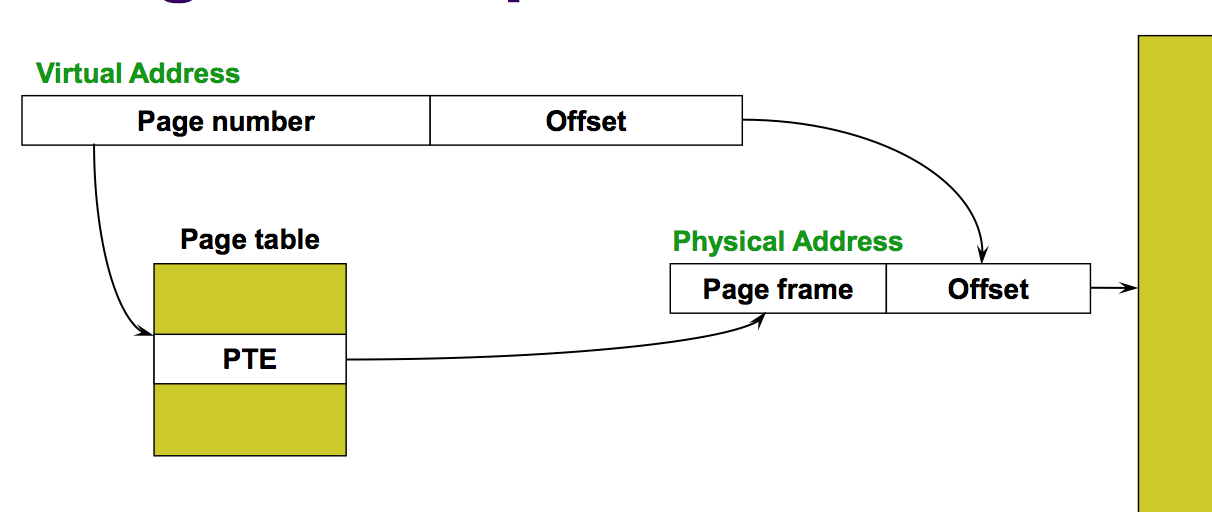
\includegraphics[scale=.50]{pagelookup}

This approach is wrong since it needs 2 references for address lookup, one for the page table and the other for the actual memory. The idea is to use hardware cache of page table entries called a \textbf{Translation Lookaside Buffer (TLB)}, which stores recently used translations.

\subsubsection{Translation Lookaside Buffer}

These translate virtual page numbers into PTEs (not phyiscal addresses), and can be done in a single machine cycle.\\
\\
TBLs are implemented in hardware with Fully associative cache (so that all entries are looked up in parellel, cache tags are virtual page numbers, cache values are PTEs). With the Page table entry and the offset, we can directly calculate the physical address.\\
\\
TLBs are small, only varying from 64-1024 entries, and address translations for most instructions are handled using the TLB (~99\%). If the PTE is found in the TLB, this is called a \textbf{TLB Hit}, and if it isn't and the page table in memory needs to be checked, this is called a \textbf{TLB Miss}.
\\
\\
TLBs are effective because of locality, Processes only use a handful of pages at a time and so we only need to "map" those pages. Hit rates are therefore very important.

\subsubsection{Managing TLBs}

Who places translations into the TLB?\\
\\
(Hardware Solution) The Memory Management Unit knows where page tables are in main memory, and are accessed by the MMU directly as the OS maintains the tables. Tables also have to be in a hardware defined format for the MMU.\\
\\
(Software Solution) The OS places them. The TLB faults to the OS, the OS finds the appropriate PTE, and loads it into the TLB. This however, must be fast, and the CPU ISA has instructions for manipulating the TLB. In this solution, tables can be in any format convenient for the OS.\\
\\
The OS ensures that the TLB and page tables are consistent, so that when it changes the protection bits of a PTE, it needs to invalid that same PTE if it is in the TLB.\\
\\
TLBs are reloaded on a process context switch, and since it's more efficient to just invalidate all the entries instead of selecting specific ones, that is done on a context switch.\\
\\
When the TLB misses and a new PTE has to be loaded, the cached PTE must be evicted. Choosing a PTE to evict is called the \textbf{TLB replacement policy}, and is implemented in hardware, and is often very simple.

\newpage

\section{Tuesday, June 12, 2018}

\subsection{Paging}

What happens if not all pages of all processes fit into physical memory?\\
\\
Then the process is moved into the \textbf{swap space} on the disk.\\
\\
What happens if the page is evicted from main memory?\\
\\
The PTE in the page table will be set to invalid, the page will be relocated to the swap space and another PTE will store the page's location in swap space.

\subsection{Page Table Management}

How much space does a page table take up?\\
\\
From around 100MB to almost 16 PB (16 million GB) for a page table. To solve this space issue we have
\begin{itemize}
    \item Hierarchical (multi-level) page tables
    \item Hashed page tables
    \item Inverted Page tables
\end{itemize}

How can we reduce space overhead?\\
\\
Observation: We only need to map the portion of the address space actually being used (which is a tiny fraction of the entire address space), so we might be able to use this to solve that problem.
\\
\\
How do we only map what is being used?
\\
\\
We can do this by dynamically extending the page table when we need it. Note that this does not work if the address space is sparse (suffering a lot of internal fragmentation).
\\
\\
We can use another level of indirection: two-level page tables, or generally, multi-level page tables
\\
\\
Now consider a PCB in the virtual address space with only a bit of space being used by the stack and the heap. This means that the space in between the stack and heap is unused. How does address translation work now?\\
\\
\subsubsection{Multilevel Page Tables (MLPT)}

The idea is that the top level of a MLPT would redirect to secondary page tables and so on.\\
\\
So in Two-level Page Tables, the Virtual Addresses (VAs) have three parts.
\begin{itemize}
    \item A \textbf{Master page number} that maps VAs to the secondary page table
    \item A \textbf{Secondary page number} that maps page numbers to a physical frame
    \item An \textbf{Offset} that specifies an address within the physical frame
\end{itemize}

\textbf{\underline{Example:}}\\
Consider a 32-bit virtual address space, with 4K pages, which requires 12 bits. So the offset is 12 bits, leaving us with 20 left. We want the master and the secondary page tables in 1 page each, so the master page table is in a page of 4K and the secondary page table is in a page of 4K, and since page table entry is 4 bytes, we can fix a maximum of
$$4,000 / 4 = 1,000$$
entries in each page table. And since 10 bits are required to display $1,000$ entries for both the master page table and the secondary page table, then we have a perfect fit.\\
\\
This is because the master page identifier is 10-bits, the secondary page table identifier is 10 bits, and the offset is 12 bits. So in total, it is 32 bits, which is how much we have.

\subsection{Inverted Page Tables}

These keep one table with an entry for each physical page table. Entries record which virtual page number is stored in that frame as well as the process ID.\\
\\
This takes up less space, but lookups are slower. References use virtual addresses, and the table is indexed by physical addresses. We can use hasing to reduce the search time.

\subsection{Efficient Translations}

Our original page table scheme already doubled the cost of doing memory lookups. One lookup into the page table, another to fetch the data.\\
\\
Two-level page tables triple the cost. Two lookups into the page tables, a third to fetch the data, and this assumes the page table is in memory.\\
\\
TLB's hide the cost for frequently-used pages.

\subsection{Page allocation and eviction}
What happens when a new page is allocated?\\
\\
Initially pages are allocated from memory. When memory fills up, some other page needs to be evicted from memory. This is why physical memory pages are called "frames".\\
\\
Then evicted pages go to disk (the swap file). When it evicts a page, the OS sets the PTE as invalid and stores the location of \underline{the page in the swap file} in the PTE

\subsection{Page Faults}

What happens when a process accesses a page that has been evicted?

\begin{enumerate}
    \item When a process accesses the page, the invalid PTE will cause a trap (page fault).
    \item The trap will run the OS page fault handler
    \item Handler uses the invalid PTE to locate page in swap file
    \item Reads page into a physical frame, updates PTE to point to it
    \item Restarts process
\end{enumerate}

\subsection{Policy Decisions}

Page tables, MMU, TLB, etc. are mechanisms that make virtual memory possible. We'll look at policies of virtual memory management:

\paragraph{Fetch Policy} when to fetch a page
\paragraph{Placement Policy} where to put the page
\paragraph{Replacement Policy} what page to evict to make room?

\subsection{Fetch Policy}

\subsubsection{Demand Paging}
\textbf{Demand Paging} is looking at pages in the swap space in the disk when it is needed.\\
\\
The process can only page fault on one page at a time in this scenario, so when the process does a read, the Disk receives a single page-sized read request

\subsubsection{Prepaging (aka Prefetching)}

This method is predicting what future pages will be used at time of current fault and loading all of them, however, we may not know on which variables to base our predictions on and what to do if the predictions are wrong.

\subsection{Placement Policy}
In paging systems, memory management hardware can translate any virtual-to-physical mapping equally well. Why would we prefer some mappings over others?
\paragraph{NUMA (non-uniform memory access) multiprocessors} Any processor can access the entire memory, but local memory is faster.

\paragraph{Cache performance} Choosing physical pages to minimize cache conflicts.

\subsection{Replacement Policy}
What page to evict to make room?
\subsubsection{Evicting the best page}

The goal of the replacement algorithm is to reduce the fault rate by selecting the best "victim" page to remove. Replacement algorithms are evaluated on a reference string by counting the number of page faults. Note that a reference string has records of pages and number of page faults.

Let's start by assuming that we know the reference string, then what is the best replacement policy in this case?

We know that the best page to evict is the one that is never used again, and because of this, there will never be a fault on it. We also know that never is a long time, so picking the page closest to never is the next best thing. Evicting the page that won't be used for the longest period of time minimizes the number of page faults.

\paragraph{Cold Misses} When a page is referenced for the first time (this is unavoidable)

\paragraph{Capacity Misses} Caused by replacement due to limited size of memory.

\subsubsection{Belady's Algorithm (aka OPT aka MIN)}

This algorithm is known as the optimal page replacement algorithm because it has the lowest fault rate for any page reference stream.\\
\\
The idea is that we replace the page that will not be used for the longest period of time, the problem however is that we have to know the future perfectly.
\\
\\
Belady's algorithm is still useful as it is used as a guide to compare implementations of page replacement algorithms with the optimal to gauge room for improvement. i.e. If the optimal is not much better, then the algorithm is pretty good, otherwise, the algorithm could use some work. Note that Random replacement is often the lower bound.

\subsubsection{What are possible replacement algorithms?}

\begin{itemize}
    \item (FIFO) First-in-first-out
    \item (LRU) Least-recently-used
    \item Least-frequently-used
    \item Most-frequently-used
\end{itemize}

Many of these require book-keeping.

\subsubsection{Not-Recently-Used (NRU)}

We divide the pages into 4 classes:
\begin{enumerate}
    \item Not referenced, not modified
    \item Not referenced, modified
    \item Referenced, not modified
    \item Referenced, modified
\end{enumerate}

And we remove pages at from from lowest-numbered class that is not empty.

\subsubsection{First-In-First-Out (FIFO)}

FIFO is an obvious algorithm and simple to implement. We just need to maintain a list of pages in order in which they were paged in, on replacement, we evict the one brought in the longest time ago.\\
\\
This might be good because maybe the one brought in the longest ago is not being used, but this may also be bad as we don't have any info to say one way or the other.\\
\\
FIFO suffers from "Belady's Anomaly", which is that the fault rate might actually increase when the algorithm is given more memory (this is very bad).

\subsubsection{Second-Chance}

The idea is that FIFO only considers age and NRU only considers usage, maybe we should combine the two.\\
\\
The algorithm is that we don't evict the oldest page if it has been used but evict the oldest page that has not been used.\\
\\
Pages that are used often enough to keep reference bits set will not be replaced.

\subsubsection{Second-Chance Implementaiton}

We want to replace the page that is "old enough". We do this by arranging all of the physical page frames in a big circle (like a clock) and we sweep through the pages in a circular order like a clock, and if the reference bit is off, that means it has not been used recently and we exict that page. If there reference bit is on, that means it has been used recently and we turn it off to go to the next page. So the clock hand moves quickly when pages are needed, and there is low overhead when there is plenty of memory.

\subsection{Eviction Algorithms}

\subsubsection{Least Recently Used (LRU)}

LRU uses reference information to make a more informed replacement decision. The idea is that we can't predict the future, but we can make a guess based upon past experience. On replacement, we evict the page that has not been used for the longest time in the past, which is Belady's future.\\
\\
To implement this, we need to timestamp every page, and sort them to get the LRU page.
\\
\\
Well, the first problem is that we need to sort every time we evict, and where do we store the timestamp? That's something we have to store for every page. Sorting can also be costly.
\\
\\
We can try keeping pages in a stack, on reference, move a page to the top of the stack, and on eviction, replace page at the bottom, but is also very costly to manipulate stack on every memory reference.\\
\\
We don't implement the exact LRU, but we can use approximations by the PTE reference bit. The basic idea is that initially, all $R$ bits are zero; as processes execute, bits are set to 1 for pages that are used, so we periodically examine the R bits, we do not know order of use, but we know pages that were or were not used.\\
\\
Additionally, we can also have a reference bit algorithm where we keep a counter for each page, and at regular intervals, for each page, we shift the $R$ bit into highest bit of counter register, and then shift all the bits to the right, and pages with "larger" counters were used more recently.

\subsubsection{Counting-based replacement}

You can also count the number of uses of a page, here are the uses:
\paragraph{Least-Frequently-Used (LFU)} Replace the page used least often, pages that are heavily used at one time tend to stick around even when not needed anymore. Newly allocated pages haven't had a change to be used much though.

\paragraph{Most-Frequently-Used (MFU)} This algorithm favours new pages. This fixes the problem in LFU.

Neither of them is common, both are poor approximations of OPT.

\subsubsection{Comparing Replacement Algorithms}

\begin{center}
 \begin{tabular}{||c c c||}
 \hline
 Algorithm Name & Ease of Implementation & Performance \\ [0.5ex]
 \hline\hline
 Not Recently Used & Good & Ok \\
 \hline
 First In First Out & Good & Ok\\
 \hline
 Least Recently Used & Bad & Very Good\\
 \hline
 Least Frequently Used & Bad & Bad\\
 \hline
 Most Frequently Used & Bad & Bad\\
 \hline
 Second Chance & Good & Good\\ [1ex]
 \hline
\end{tabular}
\end{center}


\subsubsection{Fixed vs. Variable Space}

In a multiprogramming system, we need a way to allocate memory to competing processes. The problem is, how do we determine how much memory to give each process? There are two solutions.

\paragraph{Fixed Space Algorithms} Each process is given a limit of pages it can use, when it reaches the limit, it replaces from its own pages, but some processes may do well with this system while others may suffer.

\paragraph{Variable Space Algorithms} Process' set of pages grows and shrinks dynamically, however, one process can take up all the possible space, and replacement and set size are separate, so replacement is hard.

\subsubsection{Working Set Model}

How do you decide how large the fixed or variable space for a process should be?\\
\\
A Working Set of a process is used to model the dynamic locality of its memory usage. The definition is
$$WS(t,\Delta) = \{ \text{pages $P$ such that $P$ was referenced in the time interval $(t, t-\Delta)$} \}$$
$$t=\text{time}$$
$$\Delta = \text{working set window (measured in page references)}$$

A page is in the working set (WS) only if it was referenced in the last $\Delta$ references.\\
\\
The working set size is the number of pages in the working set, the number of pages referenced in the interval $(t,t-\Delta)$.\\
\\
The working set size changes with program locality. During periods of poor locality, you reference more pages, and within that period of time, the working set size is larger.\\
\\
Intuitively, we want the working set to be the set of pages a process needs in memory to prevent heavy faulting, so each process has a parameter $\Delta$ that determines a working set with few faults. We also don't want to run a process unless the working set is in memory.

\subsubsection{Working Set Problems}

There are a few problems with Working sets, such as
\begin{itemize}
  \item How do we determine $\Delta$?
  \item How do we know when the working set changes?
\end{itemize}

These questions are too hard to answer, so working sets are not used in practice as a page replacement algorithm. However, it is still used as an abstraction, as the intuition is still valid, and it's useful to understand how much memory a particular program needs (such as Firefox or Chrome).

\subsection{Page Fault Frequency}

Page Fault Frequency (PFF) is a variable space algorithm that uses a more ad-hoc approach. It monitors the fault rate for each process, and if the fault rate is above a upper threshold, we give it more memory with the idea that it will fault less, but this is not always the case as seen with FIFO and Belday's Anomaly. If the fault rate is below a low threshold, we take memory so that it might fault more, but this is not always the case.\\
\\
It's hard to use PFF to distinguish between changes in locality and changes in the size of the working set.

\subsubsection{Thrashing}

Thrashing is when more time is spent by the OS in paging data back and forth from the disk than executing the actual user programs. This means that no time is spent doing useful work (making progress).\\
\\
Page replacement algorithms avoid thrashing. Thrashing causes the system to be overcommitted, since the OS has no idea which pages should be in memory to reduce faults, and it could just be that there isn't enough physical memory for all of the processes in the system.\\
\\
The possible solutions to thrashing are swapping, which is writing out all pages of a process and then suspending it, or simply acquiring more memory.

\subsubsection{Windows XP Paging Policy}

Windows uses Local page replacement, which is a per-process FIFO system. Pages are stolen from process using more than their minimum working set. Processes start with a default of 50 pages. XP monitors page fault rates and adjust working set sizes accordingly. On a page fault, a cluster of pages around the missing page are brough into memory as well as the missing page.

\subsubsection{Linux Paging Policy}

Linux uses a global replacement, like most Unix systems. It uses a modified second-chance clock algorithm, in which pages "age" with each pass of the clock hand and pages that are not used for a long time will eventually have a value of zero.

\newpage

\section{Tuesday, July 3, 2018}




\subsection{File Systems}

\paragraph{What do file systems do?} They provide a nice abstraction of storage

\subsection{File Management Systems}

File Management Systems...
\begin{itemize}
    \item implement an abstraction (files) for secondary storage
    \item organize files logically (directories)
    \item Permit sharing of data between processes, people, and machines
    \item Protect data from unwanted access (security)
\end{itemize}

\subsection{File Concept}

A file is a named collection of data with some attributes. Attributes such as, Name, Owner, Location, Size, Protection, Creation Time, Time of Last Access

\subsection{File Types}

A file's type can be encoded in its name or contents.\\
\underline{Ex.} Windows encodes type in name
\underline{Ex.} Unix sometimes encodes type in contents, such as \#! for shell scripts

\subsubsection{File Operations}
\begin{itemize}
    \item Create
    \item Write
    \item Read
    \item Delete
    \item Open
    \item Close
    \item etc...
\end{itemize}

\subsection{File Access Methods}

General-purpose file systems support simple methods:

\paragraph{Sequential Access} Read bytes one at a time, in order. Operations are \codeword{read next} and \codeword{write next}.

\paragraph{Direct Access} Random access given a block/byte number. Operations are \codeword{read n} (byte at offset n) and \codeword{write n}\\

\underline{Ex.} Unix uses both\\
\\
Database systems support more sophisticated methods.

\subsection{Handling operations on files}

Involves searching the directory for the entry associated with the named file.\\
\\
When the file is first used actively, store its attribute info in a system-wide open-file table; the index into this table is used on subsequent operations. This implies no searching.

\subsection{Shared open files}

There are actually 2 levels of internal tables.
\begin{itemize}
    \item a \textbf{per-process table} of all files that each process has open (this holds the current file position for the process)
    \item each entry in the per-process table points to an entry in the \textbf{system-wide open-file table} (for process independent info)
\end{itemize}

\subsection{Directories}

Directories server multiple purposes

\paragraph{For users} They provide a structured way to organize files
\paragraph{For the file system} they provide a convenient naming interface that allows the implementation to separate logical file organization from physical file placement on the disk
\\
\\
Directories also store information about files (owner, permission, etc.)\\
\\
Most files support multi-level directories and naming hierarchies (such as \codeword{/}, \codeword{/usr/}, \codeword{/usr/local/})

\subsubsection{What is a directory at the OS level?}

A directory is a list of entries, names and associated \textbf{metadata}. Metadata not being data itself, but information that describes the properties of the data (such as size, protection, location, etc.)\\
\\
The Directories are usually a list that is usually unordered (effectively random). The entries are usually sorted by the program that reads the directory.
\\
\\
Directories are typically stored in files. This makes it easier as you would only need to manage one kind of secondary storage unit.

\subsubsection{Operations on Directories}

\paragraph{Search} Find a particular file within directory
\paragraph{Create file} Add a new entry to the directory
\paragraph{Delete file} Remove an entry from the directory
\paragraph{List directory} Return file names and requested attributes of entries
\paragraph{Update directory} Record a change to some file's attributes

\underline{Ex.} Unix. In Unix, directories are implemented in files, and you use file operations to create directories.\\
A C runtime library provides a higher-level abstraction for reading directories.

\subsection{Path Name Translation}

Let's say you want to open \codeword{/one/two/three}\\
\\
The file system first open \codeword{/}, which is the root directory, a well known directory that the file system can always find. They the file system searches for an entry \codeword{one} in the root directory, and then open the \codeword{one} directory and look for \codeword{two} in that directory, and then find and open the file \codeword{three}.\\
\\
Systems spend a lot of time walking directory paths, so this is why open is separate from read and write. The OS will cache prefix lookups to increase performance.

\subsection{File System Implementation}

How do file systems use the disk to store files?\\
\\
File systems define a block size, and Disk space is allocated in granularity of blocks (units of blocks).
\\
A "Master Block" determines location of the root directory (aka the partition control block, superblock). It's always at a well-known disk location and is often replicated accross the disk for reliability.
\\
A free map determines which blocks are free and which are allocated. It's usually implemented as a bitmap, one bit per block on the disk, and is also stored on the disk and cached in memory for performance.
\\
Remaining disk blocks are used to store files (and directories). There are many ways to do this.

\subsubsection{Directory Implementation}

\paragraph{Option 1: Linear List} This is a simple list of file names and pointers to data blocks, this requires a linear search to find entries, so it is easy to implement, but slow to execute. This is bad since directory operations are frequent.

\paragraph{Option 2: Hash Table}

Add a hash data structure to the linear list and we Hash the file name to get the pointer to the entry in the linear list.

\subsection{Disk Layout Strategies}

Since files span multiple disk blocks, How do you find all of the blocks for a file?

\begin{enumerate}
    \item Contiguous allocation. This is like memory, is fast, simplifies directory access, but is inflexible, causes fragmentation, and needs compaction.

    \item Linked, or chained, structure. This is where each block points to next, and the directory points to the first block, this is good for sequential access, but bad for all others

    \item Indexed structure (indirection, hierarchy). An "index block" contains pointers to many other blocks. This handles random searches better and is still good for sequential, but it may need multiple index blocks that are linked together.
\end{enumerate}

\subsubsection{Contiguous Allocation}

This just means that each file is stored in contiguously in blocks. Like how it is done in main memory.

\subsubsection{Linked Allocation}

This just means that each file can be separated and stored in different blocks, with a linked list linking the blocks together in order.

\subsubsection{Indexed Allocation: Unix Inodes}

Unix inodes implement an indexed structure for files. Each inode contains 15 block pointers, the first 12 are direct block pointers, and the last 3 are single, double, and triple indirect block pointers (meaning that the single pointer points to a inode that points to blocks, the double pointer points to an inode that points to inodes that point to blocks, etc...)

\subsubsection{Unix Inodes and Path Search}

Unix Inodes are not directories, they just describe where on the desk the blocks for a file are placed. Directories are files, so inodes also describe where the blocks for directories are placed on the disk.
\\
\\
Directory entries map filenames to inodes.
\\
\underline{Ex.} To open \codeword{/one}
\begin{enumerate}
    \item We first use the master Block to find the inode for \codeword{/} and read that inode into memory

    \item inode allows us to find data block for directory \codeword{/}

    \item Read \codeword{/}, look for the entry for \codeword{one}

    \item this entry gives us the location of the inode for \codeword{one}

    \item We read the inode for \codeword{one} into memory

    \item The inode says where the first data block is on the disk

    \item We read that block into memory to access the data in the file
\end{enumerate}

\subsubsection{Possible Directory Implementations}

The possible directory structures are single-level, two-level, tree-structured. There is also acyclic graph directories, which allows for shared directories, which means that the same file may be in 2 directories.

\subsubsection{File Links}

Sharing can be implemented by creating a new directory entry called a link, which is a pointer to another file or subdirectory. These links can be symbolic (aka soft) links or hard links.

\paragraph{Symbolic or Soft Link} Directory entry contains "true" path to the file

\paragraph{Hard links} Second directory entry identical to the first

\subsubsection{Issues with Acyclic Graphs}

With links, a file may have multiple absolute path names, this makes traversing a file system more complicated, as we should avoid traversing shared structures more than once.
\\
\\
Sharing can occur with duplication of information, but maintaining consistency is a problem. This can occur for example, when updating permissions in a directory entry with a hard link.
\\
\\
\paragraph{Deletion: When can the space allocated to a shared file be deallocated and reused?} This problem is somewhat easier to handle with symbolic link, which means that Deletion of a link is OK, but deletion of the file entry itself deallocates space and leaves the link pointers dangling.

A reference count for hard links is kept, so the file that the links point to is deleted when all referencing links are deleted.

\subsection{File Sharing}

File sharing has been around since timesharing. It's easy to do on a single machine and PCs, workstations, and networks get us there.
\\
\\
File sharing is incredibly important for getting work done. It is the basis for communication and synchronization.
\\
\\
There are two key issues when sharing files. \textbf{Semantics of concurrent access}, such as What happens when one process reads while another writes and What happens when two processes open a file for writing, and \textbf{Protection}.

\subsubsection{Protection}

File systems implement some kind of protection system that specifies who can access a file and How they can access it.
\\
\\
A protection system dictates whether given action by a given subject on a given object should be allowed.
\\
\underline{Ex.} You can read and\slash or write your files, but others cannot.

\subsubsection{Types of Access}

\begin{itemize}
    \item None
    \item Knowledge
    \item Execution
    \item Reading
    \item Appending
    \item Updating
    \item Changing Protection
    \item Deletion
\end{itemize}

\subsubsection{Representing Protection}

\paragraph{Access Control Lists (ACL)} For each object, maintain a list of subject and their permitted actions

\paragraph{Capabilities} For each subject, maintain a list of objects and their permitted actions

Think of a chart comparing Subjects to Objects containing the permissions for each relation.

\subsubsection{ACLS and Capabilities}

The approaches differ only in how the table is represented.
\\
\\
Capabilities are easier to transfer between users, as they are like keys and can handoff, it does not depend on the subject.
\\
\\
In practice, ACLs are easier to manage, they are Object-centric, easy to grant and easy to revoke. To revoke capabilities, we have to keep track of all subjects that have the capability -- a challenging problem.
\\
\\

ACLs have a problem when objects are heavily shared, because they become very large.

\subsubsection{File Buffer Cache}

Applications exhibit significant locality for reading and writing files. Due to this, the idea is that we should cache file blocks in memory to capture locality.
\\
\\
This is called the \textbf{File Buffer Cache}. This cache is system wide, used and shared by all processes. Reading from the cache makes a disk perform like memory. Even a small amount of cache (4 MB) can be very effective.
\\
\\
The Issues with it is that the file bugger cache competes with the virtual memory, and like the virtual memory, it has a limited size. This means that it will need to use replacement algorithms here (LRU is usually used)

\subsubsection{Caching Writes}

On a write, some application assume that data makes it through the buffer and onto the disk. As a result, writes are often slow, even with caching.
\\
\\
There are several ways to compensate for this

\paragraph{"write-behind"} Maintain a queue of uncommitted blocks and periodically flush the queue to the disk. This method is unreliable though.

\paragraph{Battery backed-up RAM (NVRAM)} As with write-behind, but maintain a queue in NVRAM. This option is expensive.

\paragraph{Log-structured File System} Always write contiguously at end of previous write.

\subsubsection{Read Ahead}

Many file systems implement \textbf{"read ahead"}. This is when the file system predicts that the process will request the next block and goes ahead and requests it. This can happen while the process is computing the previous block, which overlaps I\slash O with execution.
\\
\\
When the process requests the block, it will be in the cache. This compliments the on-disk cache, which also is doing read ahead.
\\
\\
For sequentially accessed files, this can be a huge positive. Unless blocks for the file are scattered across the disk, but file systems try to prevent that during allocation.

\newpage


\section{Tuesday, July 10, 2018}

\subsection{File System Implementation}

Files and directories live on \textbf{secondary storage}. Anything outside of that is \textbf{primary memory}. Secondary storage is anything that does not permit direct instruction execution or data fetch via machine load\slash store instructions. It is also persistent, as data survives during a loss of power.
\\
\\
We are focusing on the use of fixed hard magnetic disks for implementing secondary storage.

\subsection{Disk Components}

A Disk consists of an Actuator that has metal pins attached to it that are the read and write heads, the cylinder itself is made of multiple platters with an upper and a lower surface. A circle (or a fixed radius around the platter) on the disk is called a track, and a portion of an angle of the track is called a sector.

\subsection{Disk service time components}

When the Disk wants to move from one part of the disk to another, the head first moves up or down the line going from the inside to the outside of the disk. Then the disk needs to rotate to the angle it wants to go to.\\
\\
This means that sequential access is a lot faster than random access.

\subsection{Mixing workloads can be tricky}

\underline{Ex.} Suppose there are two processes. If each process are run in isolation, they get 20 MB/s disk throughput. However, if you run the two processes simultaneously, each gets only 2 MB/s.

\subsection{Components of disk access time}

Disk request performance depends on three steps

\paragraph{Seek} This is moving the disk arm to the correct cylinder. This depends on how fast a disk arm can move.

\paragraph{Rotation} This is waiting for the sector to rotate under the head. It depends on the rotation rate of the disk.

\paragraph{Transfer} This is the transferring of data from the surface into the disk controller electronics, sending it back to the host. This depends on the density

\subsubsection{Disks are Slow}

If we look at seek times,  we see that it's an average of 5-6 milliseconds each seek, and rotation speeds add an average latency of 3 milliseconds. This is very slow, so sequential access is much faster than random.

\subsection{OS design principles}

Since the disk I\slash O is slow, we want to
\paragraph{minimize the number of disk accesses} which can be done through caching
\paragraph{When using the disk, try to minimize access cost} Which particularly targets seeks and rotation. We can plan and schedule our disk requests and arrange the data to have more sequential accesses compared to random accesses.

\subsection{Disks are Messy}

Disk are messy physical devices, they are prone to errors, bad blocks, missed seeks, etc.
\\
\\
It is the job of the OS to hide this mess from higher level software.

\subsection{OS and Disk interaction}

Specifying disk requests requires a lot of info. This includes the cyclinder number, the surface number, the track number, the sector number, the transfer size, etc...
\\
\\
Modern disks are more complicated, as not all tracks have the same number of sectors and sectors are remapped, and other complications.
\\
\\
Older disks required the OS to specify all of this information, but fortunately modern drives provide a more high-level interface: \textbf{logical block addressing}

\subsection{Logical Block Addressing}

The disk exports its data as a logical array of blocks from 0 to $N$. The Disk maps logical blocks to a specific cylinder, surface, track, and sector. So the OS would only need to specify the logical block number to read and write to.
\\
\\
With this solution, the disk parameters are hidden from the OS

\subsection{Disk Scheduling}

Because seeks are so expensive, the OS tries to schedule disk requests that are queued waiting for the disk

\paragraph{FCFS (do nothing)} This is more reasonable when the queue only has a few requests, but long requests in the queue cause long waiting times.

\paragraph{SSTF (shorted seek time first)} This minimizes arm momement (seek time) and maximizes the request rate, it also favours middle blocks.

\paragraph{SCAN (elevator)} Requests are serviced in one direction until done, then the direction is reversed.

\paragraph{C-SCAN} Like SCAN, but only goes in one direction (like a type writer)

\paragraph{LOOK} Like SCAN, but only goes as far as the last request in each direction. So if the disk goes from 0-199, and the lowest number request is 5, then LOOK goes left until it gets to 5, then it goes right, but SCAN goes all the way to 0 and then it goes right.

\paragraph{C-LOOK} The Same as look, but only goes in one direction.

In general, unless there are request queues, disk scheduling does not have much impact. This is more important for servers, but less for PCs.
\\
\\
Modern Disks often do the disk scheduling themselves, usually ignoring or undoing any scheduling done by the OS. This is because disks know their layout better than the OS so they can optimize themselves better.

\subsubsection{Back to files and directories}

How does the OS implement the abstraction of files and directories on top of this logical array of disk blocks?

\subsubsection{Disk Layout Strategies}

Files span multiple disk blocks. How do you find all of the blocks for a file?

\paragraph{Contiguous Allocation} This is like memory, is fast and simplifies directory access. However, it is inflexible, causes fragmentation, and needs compaction.

\paragraph{Linked, or chained, structure} Each block points to the first. This is good for sequential access, but bad for all others.

\paragraph{Indexed structure (indirection, hierarchy)} An "index block" contains pointers to many other blocks. This approach handles random searches a lot better, and is still good for sequential. You may need multiple index blocks that are linked together though.

\subsubsection{Indexed Allocation: Unix Inodes}

Unix inodes implement an indexed structure for files. Each inode contains 15 block pointers, where the first 12 are direct block pointers (they point to data blocks) and then the last 3 will be a single indirect pointer, a double indirect pointer, and a triple indirect pointer (in which they all point to inodes).

\subsubsection{Unix Inodes and Path Search}

\paragraph{Note} Unix Inodes are not directories, they describe where on the disk the blocks for a file are placed. Directories are also files, so inodes also describe where the blocks for directories are placed on the disk.

\underline{Ex.} We need to find the first data block for the file \codeword{/one.txt}

To open \codeword{/one.txt}, we use the Master Block to find the inode for \codeword{/} on the disk and read the inode into memory. The inode then allows us to find the data block for the directory \codeword{/}, we read it, and look for the entry for \codeword{one.txt}. This entry locates the inode for \codeword{one.txt}, so we read that into memory and that inode says where the first data block is on the disk. We read that block into memory to access the data in the file.

\subsection{File System Implementation}

A "Master Block" determines the location of the root directory (aka partition control block or superblock). A free map determines which blocks are free and which are allocated. The remaining disk blocks are used to store files and directories.

\subsubsection{Original Unix File System}

Recall that the File System sees storage as a linear array of blocks, so each block has a \textbf{logical block number (LBN)} in the original Unix. This is a simple, straightforward implementation that is easy to understand, but is a poor utilization of disk bandwidth because to find a block, the file system must search through $O(n)$ blocks, where $n$ is the total number of blocks. This is slow and can be improved on.

\subsubsection{Data and Inode Placement}

The Original Unix File System had two placement problems:
\\
\\
One was that \textbf{Data blocks allocated randomly in aging file systems}. This means that blocks for the same file are allocated sequentially when the File System is new. As the File System "ages" and fills, we need to allocate blocks of a file into the blocks of freed up spaces when other files are deleted. The problem where is that deleted files are essentially randomly placed and the blocks for new files become scattered across the disk.
\\
\\
The second is that \textbf{Inodes become allocated far from blocks}. All of the inodes would be allocated at the beginning of the disk, far from the data. This implies that traversing file name paths, manipulating files and directories requires going back and forth from inodes to data blocks.
\\
\\
Both of these problems generate many long seeks.

\subsubsection{Fast File System (FFS)}

People working on BSD Unix did a redesign that they called the \textbf{Fast File System}. It improved the disk utilization and decreased the response time of Unix's File System. It is now the File System in which all other Unix Filesystems are compared to and is a good example of being device-aware for performance.

\subsubsection{Cylinder Groups}

BDS FFS addressed placement problems using the notation of a cylinder group (aka allocation groups in lots of modern Filesystems). This has the disk partitioned into groups of cylinders. Data blocks in the same file are allocated in the same cylinder group. Inodes for files allocated in the same cylinder group as file data blocks.
\\
\\
Allocation in cylinder groups provides closeness and reduces the number of long seeks.
\\
\\
However, to be able to allocate to cylinder groups, the disk must have free space scattered across cylinders. This means that 10\% of the disk is reserved just for this purpose. If a preferred cylinder group is full, we allocate space to a "nearby" group.

\subsubsection{Space Allocation in Cylinder Groups}

If possible, do allocation in groups of 8 blocks (bytes in the bitmap). We do allocation by first finding the first byte that is all zero, and we backtrack into the previous cylinder group to check for zero.

\subsubsection{More FFS Solutions}

Small blocks (around 1K) in the original Unix File System caused 2 problems: Low bandwidth utilization and small max file size.
\\
\\
This is fixed by using a larger block (4k) but has the new problem of internal fragmentation.

\subsection{The Linux Second Extended File System (EXT2)}

A blog group contains
\begin{itemize}
    \item a Super-block
    \item a Group descriptor
    \item a Bock bitmap
    \item an I-node bitmap
    \item I-nodes
    \item Data blocks
\end{itemize}

A linux directory entry has an inode number, an entry size that helps point to the index of the next entry, a type, a file name length, and then the file name.

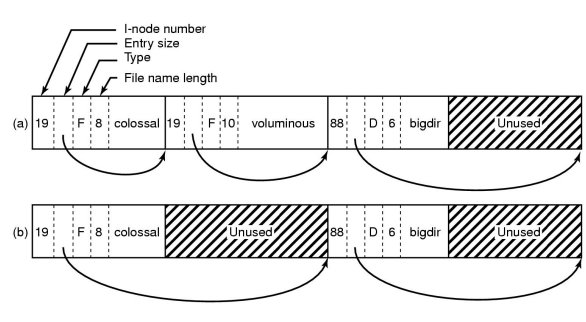
\includegraphics[scale=0.75]{yes1}\\

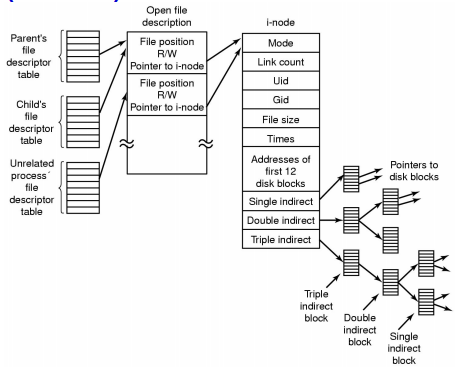
\includegraphics[scale=0.75]{yes2}
\subsection{Fast File System: Consistency Issues}

The Inodes have a fixed size structure stored in cylinder groups, and Metadata updates are synchronous operations. The operations can be placed in the wrong order as such:
\begin{itemize}
    \item Writing newly allocated inodes to the disk before its name is entered in a directory
    \item Removing a directory name before the inode is deallocated
    \item Writing a deallocated inode to disk before its blocks are placed into the cylinder group free list
\end{itemize}
\\
\\
Some updates can also create cyclical dependencies.

\subsubsection{Fast File System Observations}

If the server crashes in between any of the above synchronous operations, then the file system is in an inconsistent state.
\\
\\
The solutions to this are \textbf{fsck} which is a post-crash recovery process to scan the file system structure and restore consistency, and also log updates to enable roll-back or roll-forward.
\\
\\
The performance of the Fast File System is optimized for disk block clustering, using properties of the disk to inform system layout.
\\
\\
\underline{Observation:} Memory is now large enough that most of the reads that go to the disk are the first read of a file. Subsequent reads are satisfied in memory by file buffer cache. This means that there is no performance problem with reads, but write calls could be made much faster.
\\
\\
Writes are not well-clusted, they include inodes and data blocks.

\subsection{Log Structured File System (LSF)}

This is writing all file system data into a continuous log. This uses inodes and directories from the Fast File System. It requires an inode map to find the inodes, as an inode number is no longer a simple index.
\\
\\
There is alsoa  Cleaner that reclaims space from overwritten or deleted blocks.

\subsubsection{LFS Reads}

If the writes are now easy in this implementaiton, what happens to the reads?
\\
\\
Now, to read a file from the disk:
\begin{enumerate}
    \item We Read the superblock to find the index file
    \item We Read the index file (it's a linear search on a block of inodes)
    \item We use the disk address in the inode to read the block of the index file containing the inode map.
    \item We get the file's inodes
    \item Then we use the inode as usual to find the file's data blocks
\end{enumerate}
But remember, we expect reads to hit in memory most of the time.

\subsection{NTFS (Windows)}

The New Technology File System from Microsoft replaced the old FAST file system.
\\
\\
The designers had the following goals:
\begin{itemize}
    \item Eliminate fixed-size short names
    \item Implement a more thorough permissions scheme
    \item Provide good performance
    \item Support large files
    \item Provide extra functionality, such as Compression, Encryption and Types.
\end{itemize}

In other words, they wanted a file system that was flexible enough to support future needs.
\\
\\
Each volume (partition) is a linear sequence of blocks (usually 4KB block size). Each volume also has a Master File Table (MFT), which is a sequence of 1 KB records and contains one or more records per file or directory, so it's similar to inodes, but more flexible. Each MFT record is a sequence of variable length (attribute, value) pairs. Long attributes can be stored externally, and a pointer kept in the MFT record.
\\
\\
NTFS tries to allocate files in runs of consecutive blocks

\subsubsection{Master File Table Record}

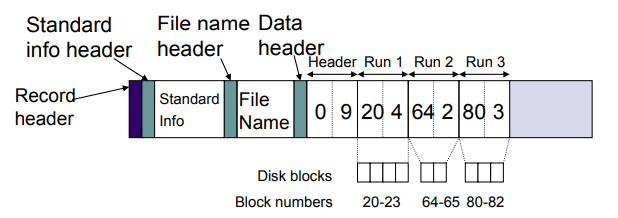
\includegraphics[scale=0.5]{yes3}

Each "data" attronite indicates the starting block and the number of blocks in a "run" (or extent). If all the records don't fit into one Master File Table record, extension records can be used to hold more.

\subsubsection{Master File Table Record for a Small Directory}

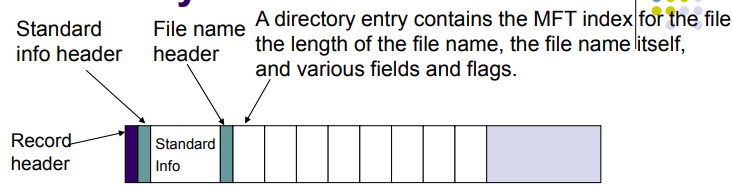
\includegraphics[scale=0.5]{yes4}

Directory entries are stored as a simple list. Large directories use B+ trees

\subsection{Better I\slash O performance through parallelism}

The Idea is that we should spread the work across several disks.

\paragraph{RAID} Redundant Arrays of Inexpensive Disks

\paragraph{RAID Level 0} Using two disks, we put half of the data on one disk and the other half on the other (this is called striping), this will double our capacity as well as read and write speeds, but if one disk fails, then data is lost, so it is not reliable

\paragraph{RAID Level 1} Using two disks again, but the data is backed up onto both of them. This has the speed for reading and writing and capacity of one disk, but if one disk fails, then the data is still there because at least half of the disks where used for redundancy.

\paragraph{RAID Level 4} Consider 5 disks, 4 are dedicated to storage and the last disk contains enough information so that if any number of the other disks fail, the last disk will be able to construct their last saved state.

\paragraph{RAID Level 5} Considering 5 disks again, now the dedicated disk for reconstructing failing disks will have its storage spread out to all the other disks.

\newpage

\section{Tuesday, July 17, 2018}

\subsection{Types of Resources}

\paragraph{Reusable} These resources can be used by one process at a time, released and used by antoher process. This includes printers, memory, processors, files, locks, semaphores, and monitors.

\paragraph{Consumable} These resources are dynamically created and destroyed, and can only be allocated once. Some examples are interrupts, signals, and messages.


\subsection{Not just an OS Problem}

There was a law passed by Kansas Legislature in the early 20th century.\\
\\
"When two trains approach each other at a corssing, both shall come to a full stop and neither shall start upon again until the other has gone"

\subsection{Deadlock Defined}

A deadlock is the \textbf{permanent} blocking of a set of processes that either compete for system resources or communicate with each other.
\\
\\
Each process in the set is blocked, waiting for an event which can only be caused by another process in the set. Key points here are that resources are finite and may be held by other waiting processes, and processes wait if a resource they need is unavailable.

\subsection{Example of a Deadlock}

Suppose processes $P$ and $Q$ need (reusable) resources $A$ and $B$.\\
\\
$P$ gets resource $A$ and $Q$ gets resource $B$, but now $P$ wants to get $B$ and $Q$ wants to get $A$, but they can't because the other process is using it.
\\
\\
If this is drawn out in a diagram, a deadlock will result in a loop.

\subsection{Dining Philosophers}

A philosopher needs two forks to eat. If the protocol for all of them is to grab the right fork and then the left fork when hungry, this can cause a deadlock. (Note that this does not guarantee a deadlock, but it can happen, for example, if the philosophers all get hungry at the same time and they all pick up their left fork, there is no more right forks to pick up and they will all be stuck in a deadlock)

\subsection{Conditions for Deadlock}

These are the necessary conditions for a Deadlock

\begin{enumerate}
  \item \textbf{Mutual Exclusion}, So that only one process may use a resource at a time
  \item \textbf{Hold and wait}, a process may hold allocated resources while awaiting to be assigned other resources
  \item \textbf{No preemption}, No resource can be forcibly removed from a process holding it.
\end{enumerate}


There is also

\paragraph{Circular Wait} which is a closed chain of processes exist, such that each process holds at least one resource needed by the next process in the chain.

Together, these 4 conditions are necessary and sufficient for a deadlock (circular wait is the only condition that is sufficient, but not necessary).

\subsection{Solutions to Deadlocks}

\subsubsection{Deadlock Prevention}

Ensure one of the 4 conditions doesn't occur
\paragraph{Preventing Mutual Exclusion} This one is not feasible, as it is often required for correctness

\paragraph{Preventing Hold and Wait} This is only getting the resources when they are all available at the same time. This is flawed as it may cause starvation due to the resources not being available all at the same time, may hold resources for a long time without using them which can block other processes. The processes may not know all resource requirements in advance, and may also have opportunities to use alternative resources, but may not take it with this opportunity. An alternative is to release all currently-held resources when a new one is needed, then make a request for the entire set of resources once again (so all the resources and the new one), but this may also cause a deadlock by rolling back their work.

\paragraph{Preventing No-Preemption} This is forcibly removing a resource from one process and assign it to another. However you may need to save the state of the process losing the resource so it can recover it later, we may need to rollback to an either state, and this method is also impossible for consumable resources.

\paragraph{Preventing Circular Waiting} Assign a linear ordering to resource types and require that a process holding a resource of one type, $R$, can only request resources that follow $R$ in the ordering.

\underline{Ex. of Preventing Circular-wait}

Let's define that $R_i$ precedes $R_j$ if $i < j$.
\\
\\
Let's consider the example of two processes, $P$ and $Q$, and resources $R_i$ and $R_j$. For a deadlock to occur, we need process $P$ to hold $R_i$ and request $R_j$, while process $Q$ holds $R_j$ and requests $R_i$.
\\
\\
If we consider these both to be true, it implies that $i<j$ from process $P$'s request and that $j<i$ from process $Q$'s request, this is impossible, so deadlocks are impossible with this method.
\\
\\
However, it can be hard to come up with a total order when there are lots of resource types

\subsubsection{Deadlock Avoidance}

All prevention strategies are unsatisfactory in some situations. \textit{Avoidance} allows the first three conditions to occur, but orders events to ensure that circular wait does not occur. This however, requires knowledge of future resource requests to decide what order to choose, and the amount and type of information varies by algorithm.
\\
\\
There are two avoidance strategies

\begin{enumerate}
  \item Do not start a process if its maximum resource requirements, together with the maximum needs of all processes already running, exceed the total system resources. This approach however, is very pessimistic, and assumes that all processes will need all their resources at the same time.

  \item Do not grant an individual resource request if it might lead to a deadlock.
\end{enumerate}

\subsubsection{Safe States}

A state is \textbf{safe} if there is at least one sequence of process executions that does not lead to deadlock, \textit{even if every process requests their maximum allocation immediately}.


\subsubsection{Unsafe States and Algorithm}

A unsafe state is one which is not safe. This is because it's just risky and a deadlock could happen, but it does not necessary imply a deadlock. It's just unsafe.
\\
\\
The \textbf{Deadlock} avoidance algorithm is as follows:
\\
For every resource request
\begin{enumerate}
    \item Update the state assuming that request is granted
    \item Check if the new state is safe
    \item If the state is safe, continue
    \item If the state is not safe, then restore the old state and block the process until it is safe to grant the request
\end{enumerate}

This is called the \textbf{Banker's Algorithm}, and in it, processes must declare their maximum needs.

\subsubsection{Restrictions on Avoidance}

Maximum resource requirements for each process must be known in advance. Processes must also be independent, so that if the order of execution is constrained by synchronization requirements, then the system is not free to choose a safe sequence.
\\
\\
Avoidance also requires a fixed number of resources to allocate.

\subsubsection{Deadlock Detection and Recovery}

Prevention and avoidance is awkward and costly. Algorithms need to be cautious, thus, will not maximize the utilization of its resources.
\\
\\
Instead, allow deadlocks to occur, but detect when this happens and find a way to break it.  So this new approach is to check for the circular wait condition periodically.
\\
\\
But how do we detect a deadlock? We draw \textbf{Resource Allocation Graphs}, and check for cycles within that. These are directed graphs where all processes and resources are nodes, and there is an edge between a process node $A$ to a resource node $B$ if process $A$ requests and is waiting for resource $B$, and there is an edge between a resource node $C$ and a process node $D$ if the resource $C$ is currently being held (or used) by a process $D$.

\subsubsection{Deadlock Recovery}

Here are solutions when a deadlock is found

\paragraph{Drastic} Kill all deadlocked processes

\paragraph{Painful} Backup and restart deadlocked processes (hopefully, non-determinism will keep the deadlock from repeating)

\paragraph{Better} Selectively kill deadlocked processes until the cycle is broken. This means re-running the detection algorithm after each kill.

\paragraph{Tricky} Selectively preempt resources until cycle is broken. However this method requires that processes must be rolled back.

\subsection{Reality Check}

No single strategy for dealing with deadlocks is appropriate for all resources in all situations. All of the strategies are costly in terms of computation overhead, or restricting use of resources.\\
\\
Most operating systems employ the \textbf{Ostrich Algorithm}, which is to ignore the problem and hope it doesn't happen again.

\subsubsection{Why does the Ostrich Algorithm Work?}

Recall the causes of a deadlock:
\begin{itemize}
    \item Resources are finite
    \item Processes wait if a resource they need is unavailable
    \item Resources may be held by other waiting processes
\end{itemize}

Prevention, Avoidance, and Detection mostly deal with the last 2 points, and Modern operating systems virtualize most physical resources, eliminating the first problem. Some logical resources can't be virtualized, such as bank accounts or the process table, these are protected by synchronization objects, which are now the only resources we can deadlock on

\subsubsection{What is atomicity?}

Consider the ATM banking example from earlier.
\\
\\
What if we needed to transfer funds between accounts? There is a withdrawal of funds from one account, and a deposit of funds into the other.
\\
\\
These operations should appear as a single \textbf{atomic} operation. Another process reading the account should see either both updates, or none. So either both operations complete, or neither does.

\subsubsection{Why would atomicity fail?}

Suppose fund transfer is implemented by our known withdraw and deposit functions using locks. What can go wrong?
\\
\\
Well lets say that the whole system crashes during the middle of the transfer is complete, this would result in only half of the work being done, which is not atomic.

\subsubsection{Definitions for Transactions}

\paragraph{Transaction} A collection of operations that performs a single logical function and are executed atomically. In this course, it involves a sequence of read and write operations terminated by a \textbf{commit} or an \textbf{abort}.

\paragraph{Committed} A transaction that has completed successfully, this means that all operations took effect. Once committed, a transaction cannot be undone.

\paragraph{Aborted} A transaction that did not complete normally. This means that none of the operations took effect

\subsubsection{How to ensure atomicity in the face of failures?}

Note that reads don't really matter, because it doesn't change anything, so only writes happen.
\\
\\
What we can do is write all intended operations to a log on a stable storage. Then we execute the actual operation. This can be used to undo\slash redo any transaction, allowing recovery from arbitrary failures.

\subsubsection{Write-ahead logging}

Before performing any operations on the data, write the intended operations to a log on stable storage. The Log records identify the transaction, the data item, and the old and new values. Special records indicate the start and commit (or abort) of a transaction. The log can then be used to undo or redo the effect of any transaction, allowing recovery from arbitrary failures.

\subsubsection{Problems with logging}

\begin{itemize}
  \item It is very time-consuming to process an entire log after a failure.
  \item Logs require a large amount of space
  \item Performance penalty -- each write requires a log update befoore the data update.
\end{itemize}

Checkpoints help with the first two problems
\begin{itemize}
  \item Periodically write all updates to log and data to stable storage; write a checkpoint entry to the log
  \item Recovery then only needs to look at the log since the last checkpoint.
\end{itemize}

\subsection{Concurrent Transactions}

Transactions must appear to execute in some arbitrary but serial order.

\paragraph{Solution 1} All transactions execute in a critical section, with a single common lock (or mutex semaphore) to protect access to all shared data. However, most transactions will access different data and this unnecessarily limits concurrency.

\paragraph{Solution 2} Allow operations from multiple transactions to overlap, as long as they don't conflict. But the end result of a set of transactions in this way must be indistinguishable from Solution 1.

\subsubsection{Confliciting Operations}

Operations in two different transactions conflict if both access the same data item and at least one is a write. Non-conflicting operations can be reordered (swapped) without changing the outcome. If a serial schedule can be obtained by swapping non-conflicting operations, then the original schedule is \textbf{conflict-serializable}.

\subsubsection{Conflict Serializability Example}

Consider two processes $T_0$ and $T_1$, lets say $T_0$ reads and writes to a file $A$, then $T_1$ reads and writes to a file $A$, then $T_0$ reads and writes to a file $B$, then $T_1$ reads and writes to a file $B$.
\\
\\
This serial execution is conflict serializable with the execution of $T_0$ doing all its operations first then $T_1$ doing all of it's operations last, since $T_1$ does all of its operations last anyways.

\subsubsection{Ensuring serializability}

\paragraph{Two-phase locking} This method includes individual data items having their own locks. Each transaction has a growing phase and a shrinking phase, but does not guarantee to be deadlock free.
\paragraph{Growing} A transaction may obtain locks, but may not release any lock
\paragraph{Shrinking} A transaction may release locks, but may not acquire any new locks.

\subsection{Timestamps}

\subsubsection{Timestamp Protocols}

Each transaction gets a unique \textbf{timestamp} before it start executing. Transactions with "earlier" timestamps must appear to complete before any later transactions.
\\
\\
Each data item has two timestamps
\paragraph{W-TS} The largest timestamp of any transaction that successfully wrote the item
\paragraph{R-TS} The largest timestamp of any transaction that successfully read the item

\subsubsection{Timestamp Ordering}

\paragraph{Read Timestamps} If the transaction has an "earlier" timestamp than W-TS on data, then transaction will end up reading a value that has already overwritten, since the read is going to happen before the write. In this case, we abort the transaction and restart with a new timestamp for read.

\paragraph{Write Timestamps} If the transaction has an "earlier" timestamp than R-TS (W-TS) on the data, then the value produced by this write should have been read (overwritten) already. We solve this by also aborting and restarting.

Note that some transactions may "starve" if repeatedly aborted and restarted.

\subsection{Deadlock and Starvation}

A set of threads is in a \textbf{deadlocked} state when ever process in the set is waiting for an event that can be caused only by another process in the set.
\\
\\
A thread suffering \textbf{starvation (or indefinite postponement)} if it is waiting indefinitely because other threads are preferred in some way.

\subsubsection{Communication Deadlocks}

Messages between communicating processes are a consumable resource.
\\
\\
\underline{Ex.}\\
Process $B$ is waiting for a request, and Process $A$ sends a request to $B$, and waits for a reply, and Process $A$'s request gets lost in the network. Then Process $B$ keeps waiting for a request and $A$ keeps waiting for a reply, this is a deadlock.
\\
\\
The solution is to use timeouts and portocols to detect duplicate messages

\subsubsection{Livelock}

"Alive, but not doing any work"
\\
\\
Occurs when a set of processes continually try some failed operation and prevent other processes in the set from making process. This is functionally equivalent to a deadlock.
\\
\\
\underline{Ex.} Consider a set of processes retrying a failed \codeword{fork()}. Let's say that the operation is done when the process table is full, so no process exits, so \codeword{fork()} keeps failing

\newpage

\section{Tuesday, July 24, 2018}

\subsection{Computer Security}

Computer Security is about techniques for computing in the presence of adversaries.

\subsubsection{Four Requirements of Secuity}

\paragraph{Confidentiality} Preventing unauthorized release of info
\paragraph{Integrity} Prevent unauthorized modification of info
\paragraph{Availability} Ensuring access to legitimiate users
\paragraph{Authenticity} Verifying the identity of a user

Cryptography gives us techniques for communicating in the presence of adversaries

\subsubsection{Types of Threats}

\paragraph{Loss of Confidentiality} Attacker gains knowledge they should not have access to
\paragraph{Attack on Integrity} Attacker alters existing files, programs, network packets, etc.
\paragraph{Attack on Availability} Theft or Denial of Service
\paragraph{Attack on Authenticity} Attacker frabricates trusted sources

\subsubsection{Vulnerabilities in the System}

\paragraph{Physical Access} unauthorized physical access makes it easy to gain unauthorized digital access
\paragraph{Humans} Who should you trust? And how much should you trust them with?
\paragraph{Operating System} Flaws in the system allows security protocols to be circumvented
\paragraph{Networks} Data travels over unsecured communication lines, across multiple administrative domains

\subsubsection{Intrusion Detection}

We generally want to know when a system has been compromised. There are two main approaches to this.

\paragraph{Signature-based Detection} Examine System Activity or Network traffic patterns that match known attacks
\paragraph{Anomaly Detection} identify patterns of "normal" behaviour over time and detect deviations from those patterns

Systems need records of user activity to help detect and recover from intrusions. These records have to be protected from tampering by the intruder.

\subsubsection{Malicious Software}

\paragraph{Trap Doors} Programs that contains a secret entry point that allows attackers to bypass security
\paragraph{Logic Bombs} Destructive code in a legitimate program triggered by some event
\paragraph{Trojan horses} Apparently useful program that tricks users into running it, but may contain a logic bomb or be a vehicle for spreading a virus
\paragraph{Virus} A program that can "infect" other programs by copying itself into them
\paragraph{Worms} A program that spreads via network connections, do not need to attach another program unlike viruses

\subsubsection{Stack and Buffer Overflow Attacks}

This is the most common means of gaining unauthorized access to a system.
\\
\\
It works by an Overflow on some stack-allocated input bugger past the space that is allocated for the input. Then overwriting the return address with the address of the exploit code, and then overwriting the next space in the stack with the exploit code itself.

\subsubsection{Trusted Computing Base (TCB)}

Think carefully about what you trust with your data.
\\
\\
If you type your password on a keyboard, you're trusting the keyboard, the computer, the OS, the password library, and the application that is checking the password. So the TCB is the set of components that you trust your secrets with.

\subsubsection{Network Communications}

Protecting "assets" on a single computer system with multiple users is hard, but dealing with networks is even harder, as they may contain Multiple administrative domains and Users of the network may not have common intersts.
\\
\\
There are two main categories of network attacks
\paragraph{Passive} eavesdropping or monitoring communication
\paragraph{Active} modification or tampering with the communication stream

\paragraph{Eavesdropping} Reading network packets that were not intended for the attacker. This does not interfere with the delivry of the messsage to its intended recipient

\subparagraph{Defense against Eavesdropping} Obfuscate message content so attacker gains no information from intercepting the message

\subsection{Encryption Keys}

Keys used for encryption and decryption can be the same or different.

\paragraph{Secret-key Cryptography} This is when the Private key is used for encryption and decryption. This results in faster encryption, but distributing the shared secret key is a problem.

\paragraph{Public-key Cryptography} This is when there is a Private key used only for encryption and a Public key for decryption. The decryption key can be published while the encryption key is kept secret, and they do not reveal each other, However this method is 1000 times slower to Secret-key Cryptography

\paragraph{Traffic Analysis} This refers to infering information based on sender and recipients of messages, size of messages, frequency of communication, etc.

\subparagraph{Defense against Traffic Analysis} Obfuscate communication pattern (i.e. make all messages the same length, all communications have the same number of messages, etc.)

\paragraph{Replay} Capture a legitimate message and re-send it later to produce an unauthorized effect

\subparagraph{Defense against Replay} Messages include a consumable item so they can't be reused.

\paragraph{Modification of Messages} Altering contents of a messages to change the effect

\subparagraph{Defense against Modification} Include message digest to detect tampering

\paragraph{Masquerade} Attacker pretends to be another entity or user.

\subparagraph{Defense against Masquerade} Digital Signatures

\subsubsection{Message Digests}

Given some input data of arbitrary length, compute a fixed length output. This is a one-way function in the sense that $y=f(x)$ is "easy" and finding $x$ given $y$ is computationally infeasible.

To detect tampering, compare digest computed on received message against digest of sent message. You would need to know the original digest though.

Sender can only encrypt or sign digest, or distribute digest separately from the message.

\subsubsection{Digital Signatures}

Provides a way to verify the origin and integrity of a message. The sender includes something with the message (or modifies the message in some way) that could only be generatede by the sender.

Public-key cryptography helps here, as decrypting using the sender's public key verifies that the sender created the message. Typically, only a message digest is signed to reduce overhead.

\subsubsection{Denial of Service}

Denial of service is when a system asset becomes unavailable to legitimate users. This is is an attack on availability, and is commonly a network attack, which overloads a server with bogus requests so that there are no resources for legitimate ones.

DDOS (Distributed Denial of Service) is when compromised computers are used as "zombies" in a coordinated attack on the victim.

\subsection{Security Design Principles}

Security is much, much more than just cryptography. If there is a fundamental flaw in the design of the system, then cryptography won't help. It's usually easier to find a bug in an implementation than to circumvent a cryptography system.

Unfortunately, system design is still as much an art as it is a science. But decades of building systems the wrong way have helped us gain some learned wisdom.

\subsubsection{Principle of Least Privilege}

Figure out exactly which capabilities a program needs to run, and grant it only those. This is not always easy.

\paragraph{Domains} A set of object and rights pairs.

\paragraph{Protection Domains} A protection domain contains processes and the processes inside of it can only operate within the domain.

\subsubsection{Principle of Least Common Mechanism} In a system with multiple users, mechanisms allowing resources to be shared by more than one user should be minimized.

\subsubsection{Protection Domains}

They can be represented by a protection matrix, but it's too costly to store such a sparse matrix. It can be done more efficiently with an Access Control List, in which each object is associated and the list contains all the domains that may access the object.

Can also use Capabilities, where each process is a list of objects that may be accessed.

\subsubsection{Bruce Scheneir: 3 waves of security attacks}

\begin{enumerate}
  \item physical attacks on wires and Hardware
  \item syntactic attacks on cryptography protocols and systems
  \item semantic attacks: humans and computers trust information that they shouldn't
\end{enumerate}

\subsubsection{Secure Sockets Layer}

This is used for secure communications, typically seen in web services. It uses both public and private key cryptography.

Communication begins with a \textbf{handshake protocol} between the client and server to establish identity, and set up session keys used to encrypt the remainder of the transmissions.

It requires an existance of a trusted Certification Authority (CA) where CA issues certificates to verify a server's identity signed with the CA's private key, and the client can verify a certificate with the CA's public key.

\subsubsection{Handshake Protocol}

Consider a client and a server.
\\
\\
So it starts by the Client sending a "hello" message to the server with the cipher suites that it can handle and the server sends one back in addition to the server certificate for the client to verify. So the client verifies the server identity. Generates a random pre-master secret key, and selects a cipher.
\\
\\
The Client then sends a session key with the selected cipher suite back to the server to switch the symmetric key encryption of the session, and the server does the same.
\\
\\
After that, the client and the server use their current session keys for the rest of their communication during that session with the current cipher suite.

\end{document}
